\chapter{Materials and Methods}
\label{chp:MaM}

%%%%%%%%%%%%%%%%%%%%%%%%%%%%%%%%%%%%%%%%%%%%%%%%%%%%%%%%%%%%%%%%%%%%%%%

This chapter covers the materials considered during this project and the methodologies applied throughout. The methodologies encompass generative design approaches such as L-Systems, CPPNs, and evolutionary algorithms. Modelling methods, specifically the FEM settings, are outlined. A detailed overview of the software pipeline is provided.

\section{Materials}

\subsection{Modelling}

The modelling of materials undergoing relatively large deformations is a non-trivial problem. Stored strain energy density may be used to compute stress in hyperelastic materials. The strain energy density is defined using invariants of strain. The three invariants are given as \citep{Kim2015}

\begin{equation}
	I_{1}=\lambda_{1}^{2}+\lambda_{2}^{2}+\lambda_{3}^{2}
\end{equation}

\begin{equation}
	I_{2}=\lambda_{1}^{2}\lambda_{2}^{2}+\lambda_{2}^{2}\lambda_{3}^{2}+\lambda_{3}^{2}\lambda_{1}^{2}
\end{equation}

and

\begin{equation}
	I_{3}=\lambda_{1}^{2}\lambda_{2}^{2}\lambda_{3}^{2}
\end{equation}

where $\lambda_{1}^{2}$, $\lambda_{2}^{2}$, and $\lambda_{3}^{2}$ are three eigenvalues. The undeformed state is used as the frame of reference. The three invariants will not change when using different coordinate systems. The three invariants must be positive for the deformation to be valid. The square root of $I_{3}$ measures the volume change of the material. $I_{3}=1$ if the material is incompressible. \citep{Kim2015}

The distortional strain energy density is defined as \citep{Kim2015}

\begin{equation}
	W_{1}\left ( I_{1},I_{2} \right )=\sum_{m+n=1}^{\infty}A_{mn}\left ( I_{1}-3 \right )^{m}\left ( I_{2}-3 \right )^{n}
\end{equation}

The Ogden model uses the principal stretches to define the distortional strain energy density as \citep{Ogden1972}

\begin{equation}
	\label{eq:om}
	W_{1}\left ( \lambda_{1},  \lambda_{2}, \lambda_{3} \right )=\sum_{i=1}^{N}\frac{\mu_{i}}{\alpha_{i}}\left ( \lambda_{1}^{\alpha_{i}} + \lambda_{2}^{\alpha_{i}} + \lambda_{3}^{\alpha_{i}} \right )
\end{equation}

where $N$, $\mu_{i}$, and $\alpha_{i}$ are material parameters. $N$ is usually three. The principal stretches are the three eigenvalues of the deformation gradient. If the material is incompressible, the three principal stresses are not independent, meaning $\lambda_{1}\lambda_{2}\lambda_{3}=1$. The shear modulus is \citep{Ogden1972}

\begin{equation}
	\mu=\frac{1}{2}\sum_{i=1}^{N}\alpha_{i}\mu_{i}
\end{equation}

The Ogden model correlates well with simple tension test data that is elongated up to 700\%. The model accommodates for slightly compressible behaviour and a nonconstant shear modulus \citep{Ogden1972, Kim2015}.

\subsection{Selection}

Compliant and elastic materials are commonly used in the construction of soft robots. Three specific silicon-based rubbers that are readily accessible and affordable were characterized by~\cite{Ellis2020}. These rubbers' Ogden material model parameters are shown in Table~\ref{tab:ogdpar}.

% Please add the following required packages to your document preamble:
% \usepackage{booktabs}
% \usepackage{multirow}
\begin{table}[H]
\centering
\caption[Ogden material model parameters]{Silicon-based rubber Ogden material model parameters \citep{Ellis2020}}
\label{tab:ogdpar}
\begin{tabular}{@{}crrr@{}}
\toprule
\multirow{2}{*}{\textbf{Parameter}} & \multicolumn{3}{c}{\textbf{Parameter Number}}                                                    \\ \cmidrule(l){2-4} 
                                    & \multicolumn{1}{c}{\textbf{1}} & \multicolumn{1}{c}{\textbf{2}} & \multicolumn{1}{c}{\textbf{3}} \\ \midrule
\multicolumn{4}{c}{\textbf{Ecoflex 00-30}}           \\ \midrule
$\mu$    & -0.0142909   & -3.64558e-06 & 9.59447e-08 \\
$\alpha$ & -5.22444     & -0.162804    & 11.3772     \\ \midrule
\multicolumn{4}{c}{\textbf{Mold Star 15 SLOW}}       \\ \midrule
$\mu$    & -6.50266e-06 & 0.216863     & 0.00137158  \\
$\alpha$ & -21.322      & 1.1797       & 4.88396     \\ \midrule
\multicolumn{4}{c}{\textbf{Smooth-Sil 950}}          \\ \midrule
$\mu$    & -0.30622     & 0.0283304    & 6.5963e-09  \\
$\alpha$ & -3.0594      & 4.59654      & 17.6852     \\ \bottomrule
\end{tabular}
\end{table}

Mold Star 15 SLOW is selected as the main material to be digitally modelled and manufactured for the purposes of the project. Mold Star 15's stiffness lies between EcoFlex and Smooth Sil's.  Mold Star 15 is selected because of its availability and physical properties. Mold Star 15 is deliverable to the premises where testing is to be done and available from a registered supplier. It is suitable for inflation while being capable of supporting itself at the relevant scale of construction. Additional relevant properties are listed in Table~\ref{tab:msp}.

% Please add the following required packages to your document preamble:
% \usepackage{booktabs}
\begin{table}[H]
\centering
\caption[Mold Star 15 material properties]{Additional Mold Star 15 SLOW material properties \citep{MoldStar}}
\label{tab:msp}
\begin{tabular}{@{}lr@{}}
\toprule
\multicolumn{1}{c}{\textbf{Property}} & \multicolumn{1}{c}{\textbf{Value}} \\ \midrule
Pot life (\si{\minute})                        & 50                                 \\
Cure time (\si{\minute})                       & 240                                \\
Tensile strength (\si{MPa})                & 2.7579                             \\ \bottomrule
\end{tabular}
\end{table}

Mold Star 15's long pot life allows for adequate time to prepare specimens thoroughly. Mold Star 15's relatively short cure life prevents long delays while waiting for specimens to cure. Mold Star 15's relatively high tensile strength prevents tears or ruptures at significant deformations.

\subsection{Mixing and Casting}
\label{ssec:mac}

Mold Star 15 as provided by the manufacturer consists of two components: Mold Star 15-A and Mold Star 15-B. Mold-Star 15-A is white in colour while Mold Star 15-B is blueish-green. The two components remain liquid when exposed to air or other surfaces. When mixed with each other, the components' pot life begins and the mixed material will begin to set. However, unless mixed adequately in the correct amounts, the material properties will differ from those specified and it may not set entirely.

The two components of the material need to be mixed according to a 1:1 mass ratio. A clean mixing bowl is placed on an electronic scale and the scale is zeroed. Mold-Star 15-A is added to the bowl according to half the desired amount of Mold-Star 15. The mass of Mold Star 15-A is carefully noted and the scale is zeroed again. An equal amount of Mold Star 15-B is added to the mixing bowl.

A clean disposable stirrer such as a tongue depressor is used to mix the two Mold Star components thoroughly. The mixture is considered to be thorough when it is one uniform colour and no lighter or darker streaks are visible.

The mixture must be degassed to remove any air bubbles formed during pouring or mixing. The mixture in the bowl is placed inside a degasser and the pressure is lowered to a vacuum pressure. Bubbles will rise to the top of the mixture and pop. When no bubbles have appeared for a minute, the mixture is considered degassed. It may be removed from the degasser once the pressure has equalised.

The mixture may now be cast into a mould. Care must be taken during casting to prevent the formation of more bubbles. If the mould is movable and fits within the degasser, this may be done to remove any extra bubbles formed during casting.

If the mould is open, the material must be levelled to remove excess material and prevent any menisci from forming, which would affect the specimen's thickness. The material is levelled by applying a scraper across the surface slowly. If the scraper is moved too fast, it may remove too much material, as the mixture is viscous and sticky. If the surface area is too large, a flat cover may be applied by slowly lowering it at an angle.

According to Mold Star 15's pot life, the process detailed above must be completed within \SI{45}{\minute}. The cast specimen will be ready \SI{4}{\hour} after the pot life has ended.

\section{Pattern Generation}

A component of the generative design process of this project is the construction of internal geometries. The project scope is limited to a 2D grid of squares. Pattern generation methods capable of evolving are implemented in order to generate initial geometries and improve upon them.

\subsection{L-Systems}
\label{ssec:LS}

L-Systems are implemented in the code pipeline as a pattern generation method. L-Systems are implemented according to a context-free L-System structure as defined by~\cite{Prusinkiewicz2004}. Stochastic L-Systems are not implemented to maintain replicability. Parametric L-Systems are not implemented because a single discrete model state is desirable. Maps are not implemented as the resulting reflections when branches collide with the border wall may negatively impact the scalability of the L-Systems. Reflections inward may quickly fill up the available space or result in geometries dissimilar to ones resulting from the same L-System at higher resolutions. Interactions between elements drawn are also not considered.

The L-System unit generation method is implemented due to the features of efficiency, compactness and scalability. L-Systems are defined in the Python code using class objects containing all necessary information.

\subsubsection{Parameters}

The L-System vocabulary is defined as a class object in the Python code. The vocabulary is predefined. It consists of variables and constants. The vocabulary and its interpretations are outlined in Tables~\ref{tab:lsvarint} and~\ref{tab:lsconint}. The vocabulary is separated according to variables and constants. The vocabulary interpretation differs from traditional L-System interpretations. The interpretation is required to fill in elements of a grid. Traditional L-System interpretations result in lines of varying lengths and angles being drawn. A unique interpreter was designed and implemented for the purposes of this project.

% Please add the following required packages to your document preamble:
% \usepackage{booktabs}
\begin{table}[H]
\centering
\caption{L-System variable interpretation}
\label{tab:lsvarint}
\begin{tabular}{@{}cl@{}}
\toprule
\textbf{Variable} & \multicolumn{1}{c}{\textbf{Interpretation}}                                                         \\ \midrule
F & \begin{tabular}[c]{@{}l@{}}Create an element at the current position and increment\\ the current position in the current direction\end{tabular} \\ \midrule
f                 & Increment the current position in the current direction                                             \\ \midrule
+                 & Rotate the current direction by \SI{45}{\degree} clockwise        \\ \midrule
-                 & Rotate the current direction by \SI{45}{\degree} counterclockwise \\ \bottomrule
\end{tabular}
\end{table}

% Please add the following required packages to your document preamble:
% \usepackage{booktabs}
\begin{table}[H]
\centering
\caption{L-System constant interpretation}
\label{tab:lsconint}
\begin{tabular}{@{}cl@{}}
\toprule
\textbf{Constant} & \multicolumn{1}{c}{\textbf{Interpretation}}                                                                                \\ \midrule
{[}               & Push the current position to the position memory stack                                                                     \\ \midrule
{]}               & \begin{tabular}[c]{@{}l@{}}Pop the latest position on the position memory stack\\ and return to that position\end{tabular} \\ \midrule
( &
  \begin{tabular}[c]{@{}l@{}}Push the current position to the position memory stack.\\ All directional variables, i.e. "+" and "-", in the word\\ following this constant are reversed until the ")"\\ constant is encountered\end{tabular} \\ \midrule
)                 & \begin{tabular}[c]{@{}l@{}}Pop the latest position on the position memory stack\\ and return to that position\end{tabular} \\ \bottomrule
\end{tabular}
\end{table}

Randomly generated L-Systems are manipulated using a random generation seed. Randomly generated L-Systems have requirements and specifications implemented to ensure the validity of the L-System.

At least one L-System rule must be defined. This rule must apply to the variable "F" and must itself contain at least one instance of the letter "F". Up to three additional rules may be defined, one for each of the remaining variables.

Rule components are selected from a predefined list included in Table~\ref{tab:lsrulecom}. Rule components were selected for various reasons. Rule components containing more than one character allow for variability in rule length. Rule components containing two identical directional variables specify \SI{90}{\degree} rotations. Rule components enclosed within square brackets allow for branches to exist within the L-System.

% Please add the following required packages to your document preamble:
% \usepackage{booktabs}
\begin{table}[H]
\centering
\caption[L-System rule components]{L-System rule components and their interpretations}
\label{tab:lsrulecom}
\begin{tabular}{@{}ccl@{}}
\toprule
\multicolumn{1}{l}{\textbf{Number}} &
  \textbf{\begin{tabular}[c]{@{}c@{}}Rule\\ Component\end{tabular}} &
  \multicolumn{1}{c}{\textbf{Interpretation}} \\ \midrule
1 &
  F &
  \begin{tabular}[c]{@{}l@{}}Create an element at the current position and\\ increment the current position in the current\\ direction\end{tabular} \\ \midrule
2 &
  f &
  \begin{tabular}[c]{@{}l@{}}Increment the current position in the current\\ direction\end{tabular} \\ \midrule
3 &
  + &
  Rotate the current direction by \SI{45}{\degree} clockwise \\ \midrule
4 &
  - &
  \begin{tabular}[c]{@{}l@{}}Rotate the current direction by \SI{45}{\degree}\\ counterclockwise\end{tabular} \\ \midrule
5 &
  ++ &
  Rotate the current direction by \SI{90}{\degree} clockwise \\ \midrule
6 &
  -- &
  \begin{tabular}[c]{@{}l@{}}Rotate the current direction by \SI{90}{\degree}\\ counterclockwise\end{tabular} \\ \midrule
7 &
  fF &
  2, then 1 \\ \midrule
8 &
  Ff &
  1, then 2 \\ \midrule
9 &
  {[}F{]} &
  \begin{tabular}[c]{@{}l@{}}Push the current position to the position\\  memory stack, then 1, then pop the latest\\ position on the position memory stack and\\ return to that position\end{tabular} \\ \midrule
10 &
  {[}f{]} &
  \begin{tabular}[c]{@{}l@{}}Push the current position to the position\\ memory stack, then 2, then pop the latest\\ position on the position memory stack and\\ return to that position\end{tabular} \\ \midrule
11 &
  {[}+F{]} &
  \begin{tabular}[c]{@{}l@{}}Push the current position to the position\\ memory stack, then 3, then 1, then pop the\\ latest position on the position memory stack\\ and return to that position\end{tabular} \\ \midrule
12 &
  {[}+fF{]} &
  \begin{tabular}[c]{@{}l@{}}Push the current position to the position\\ memory stack, then 3, then 7, then pop the\\ latest position on the position memory stack\\ and return to that position\end{tabular} \\ \midrule
13 &
  {[}-F{]} &
  \begin{tabular}[c]{@{}l@{}}Push the current position to the position\\ memory stack, then 4, then 1, then pop the\\ latest position on the position memory stack\\ and return to that position\end{tabular} \\ \midrule
14 &
  {[}-fF{]} &
  \begin{tabular}[c]{@{}l@{}}Push the current position to the position\\ memory stack, then 4, then 7, then pop the\\ latest position on the position memory stack\\ and return to that position\end{tabular} \\ \bottomrule
\end{tabular}
\end{table}

During initial trials, issues were encountered in allowing rules to be generated with completely random variables and constants. Unmatched brackets did not allow for the correct interpretation of the axioms. Without forcing the inclusion of the "F" character in at least one rule or applying at least one rule to the "F" character, many L-Systems did not result in the creation of any elements. If constants were treated as variables, the brackets could also end up unmatched.

Twelve axioms are predefined and outlined in Table~\ref{tab:lsaxiom}. Axioms were defined according to desirable symmetry conditions. Symmetry conditions are illustrated in Figure~\ref{fig:lssym} according to the reference shape in Figure~\ref{fig:lssymex}.

% Please add the following required packages to your document preamble:
% \usepackage{booktabs}
\begin{table}[H]
\centering
\begin{tabular}{@{}lcc@{}}
\toprule
\multicolumn{1}{c}{\textbf{Axis}}                                        & \textbf{Rotational Axiom}           & \textbf{Reflective Axiom}   \\ \midrule
Horizontal        & {[}F{]}++++{[}F{]}   & {[}F{]}++++(F)   \\
Vertical          & -{}-{[}F{]}++++{[}F{]} & -{}-{[}F{]}++++(F) \\
\begin{tabular}[c]{@{}l@{}}Horizontal and\\ vertical\end{tabular}        & {[}F{]}++{[}F{]}++{[}F{]}++{[}F{]}  & {[}F{]}++(F)++{[}F{]}++(F)  \\
Diagonal          & +{[}F{]}++++{[}F{]}  & +{[}F{]}++++(F)  \\
Negative diagonal & -{[}F{]}++++{[}F{]}  & -{[}F{]}++++(F)  \\
\begin{tabular}[c]{@{}l@{}}Diagonal and\\ negative diagonal\end{tabular} & +{[}F{]}++{[}F{]}++{[}F{]}++{[}F{]} & +{[}F{]}++(F)++{[}F{]}++(F) \\ \bottomrule
\end{tabular}
\caption{L-System axioms}
\label{tab:lsaxiom}
\end{table}

\begin{figure}[H]
	\centering
	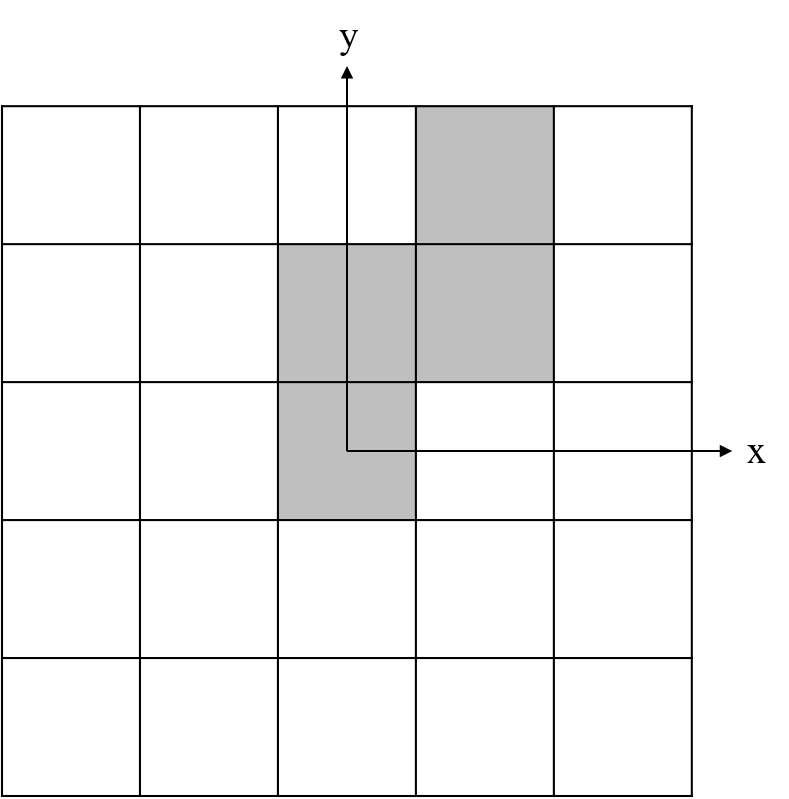
\includegraphics[width=0.5\textwidth]{LSSym.png}
	\caption[L-System symmetry reference]{L-System symmetry interpretation reference layout}
	\label{fig:lssymex}
\end{figure}

\begin{figure}[H]
	\centering
	\begin{subfigure}[t]{0.3\textwidth}
		\centering
		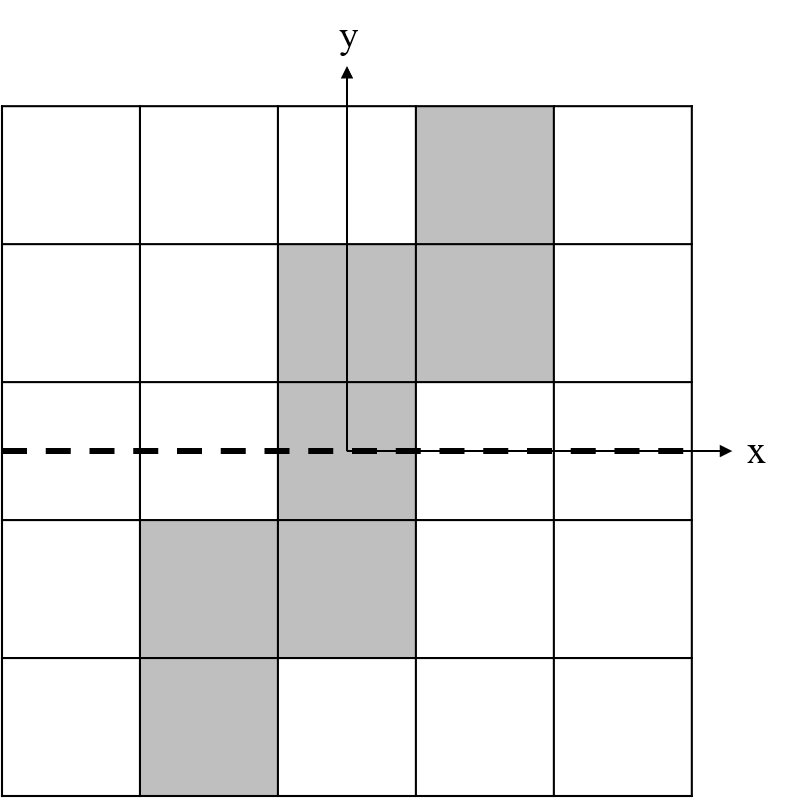
\includegraphics[width=\textwidth]{LSSymRotH.png}
		\caption{Horizontal rotation}
	\end{subfigure}
	\hfill
	\begin{subfigure}[t]{0.3\textwidth}
		\centering
		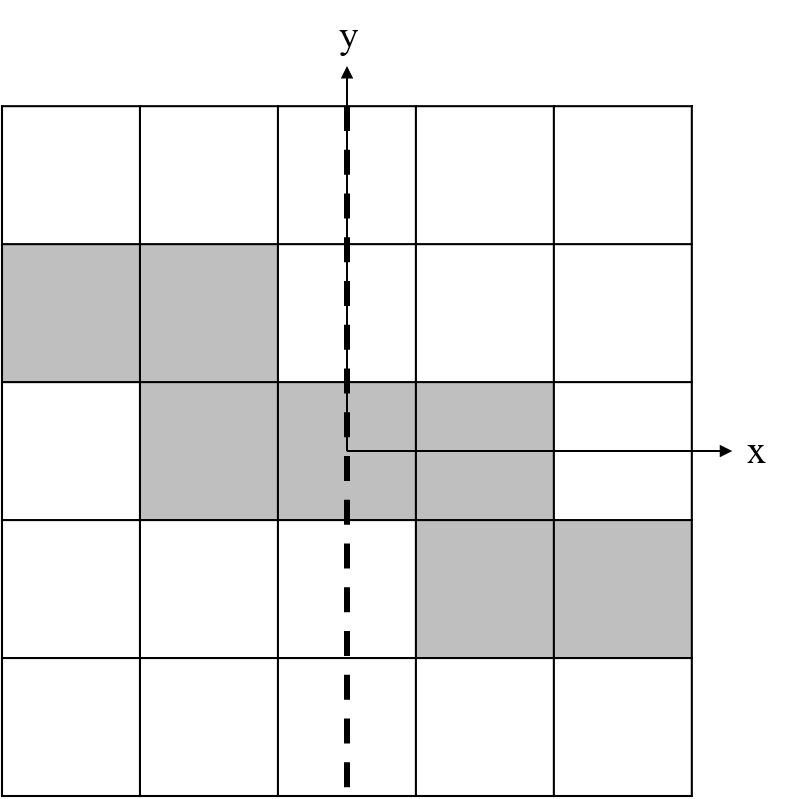
\includegraphics[width=\textwidth]{LSSymRotV.png}
		\caption{Vertical rotation}
	\end{subfigure}
	\hfill
	\begin{subfigure}[t]{0.3\textwidth}
		\centering
		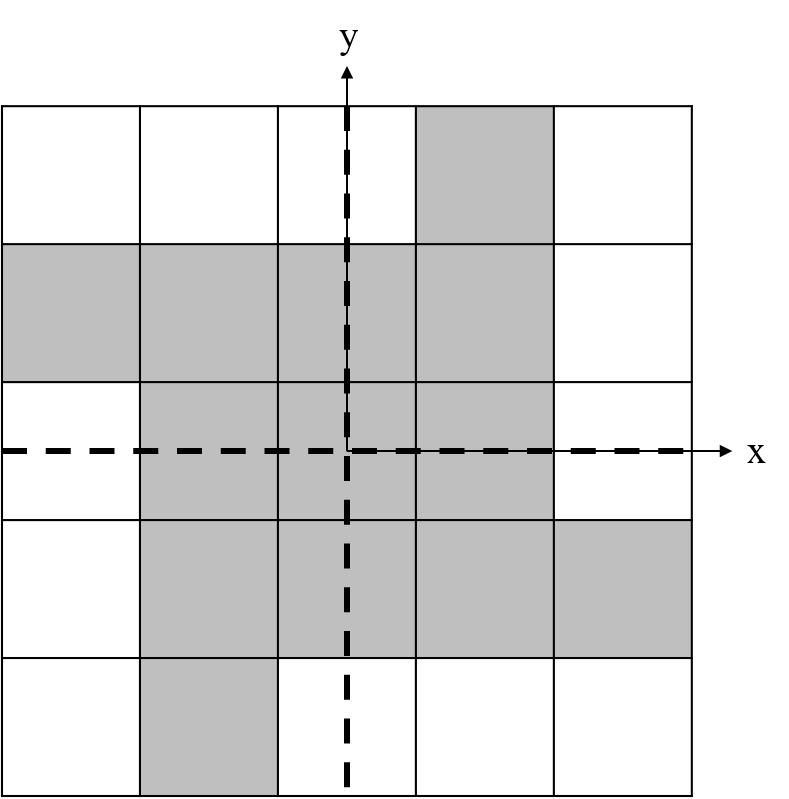
\includegraphics[width=\textwidth]{LSSymRotHV.png}
		\caption{Horizontal and vertical rotation}
	\end{subfigure}
	\hfill
	\begin{subfigure}[t]{0.3\textwidth}
		\centering
		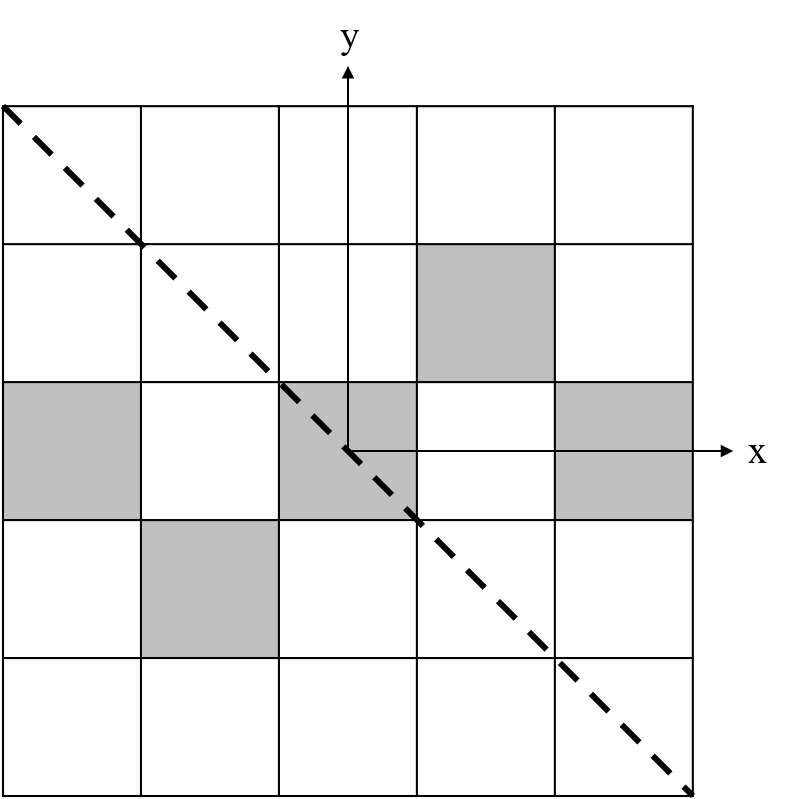
\includegraphics[width=\textwidth]{LSSymRotD.png}
		\caption{Diagonal rotation}
	\end{subfigure}
	\hfill
	\begin{subfigure}[t]{0.3\textwidth}
		\centering
		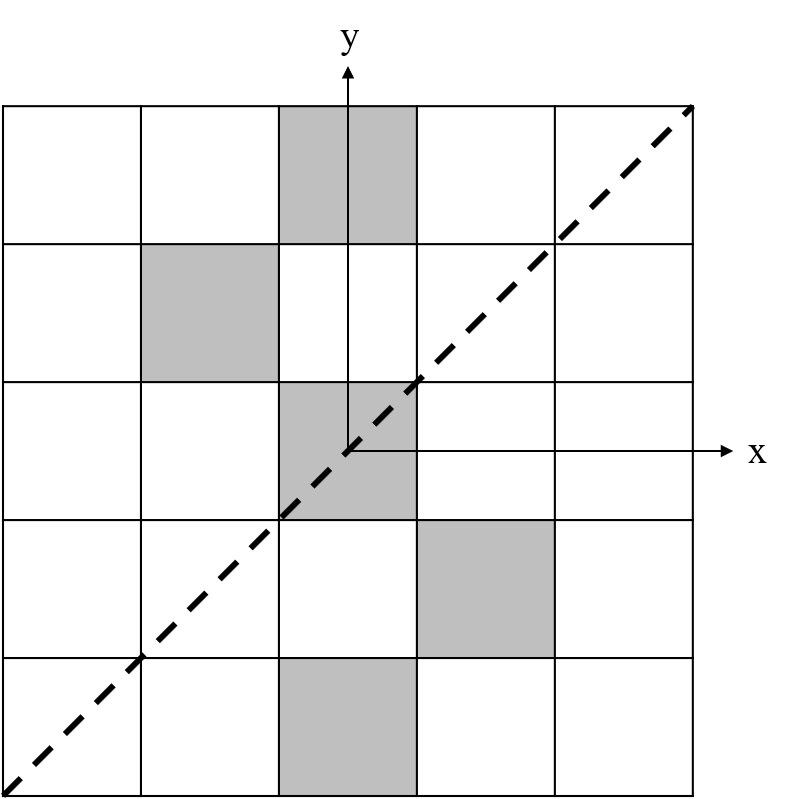
\includegraphics[width=\textwidth]{LSSymRotND.png}
		\caption{Negative diagonal rotation}
	\end{subfigure}
	\hfill
	\begin{subfigure}[t]{0.3\textwidth}
		\centering
		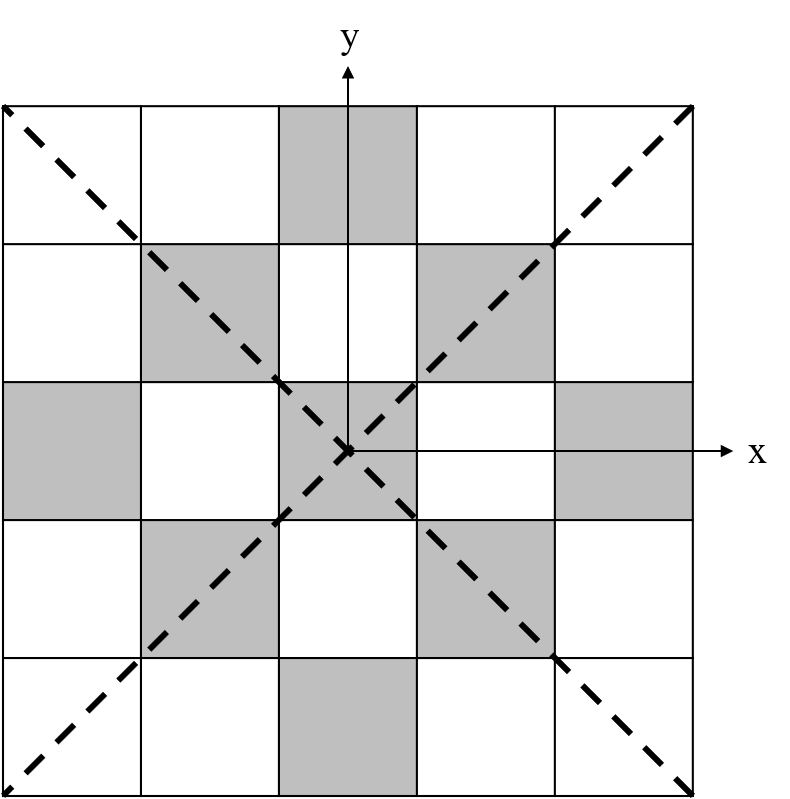
\includegraphics[width=\textwidth]{LSSymRotDND.png}
		\caption{Diagonal and negative diagonal rotation}
	\end{subfigure}
	\hfill
	\begin{subfigure}[t]{0.3\textwidth}
		\centering
		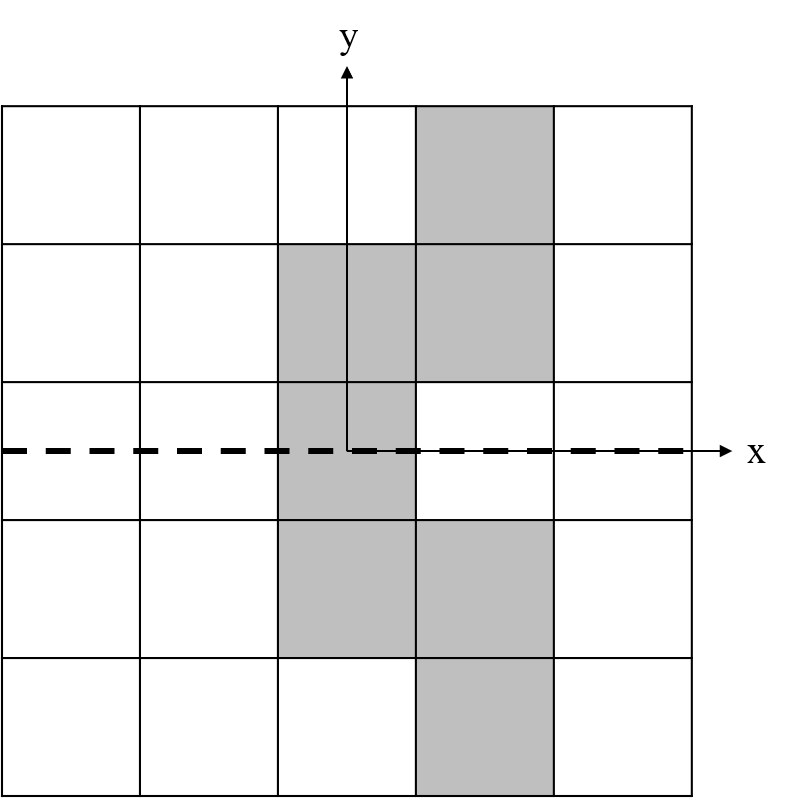
\includegraphics[width=\textwidth]{LSSymRefH.png}
		\caption{Horizontal reflection}
	\end{subfigure}
	\hfill
	\begin{subfigure}[t]{0.3\textwidth}
		\centering
		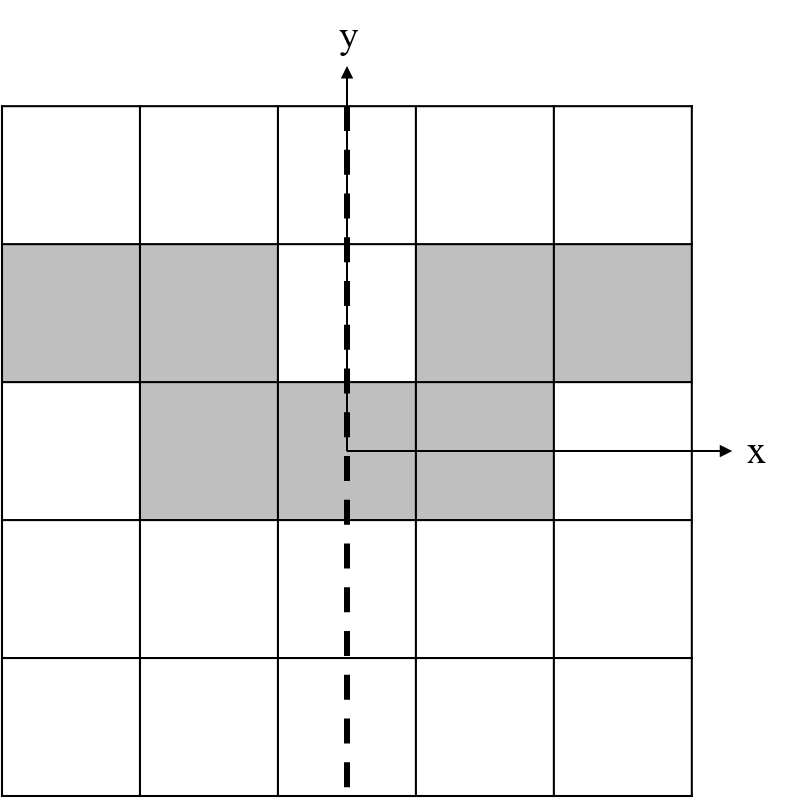
\includegraphics[width=\textwidth]{LSSymRefV.png}
		\caption{Vertical reflection}
	\end{subfigure}
	\hfill
	\begin{subfigure}[t]{0.3\textwidth}
		\centering
		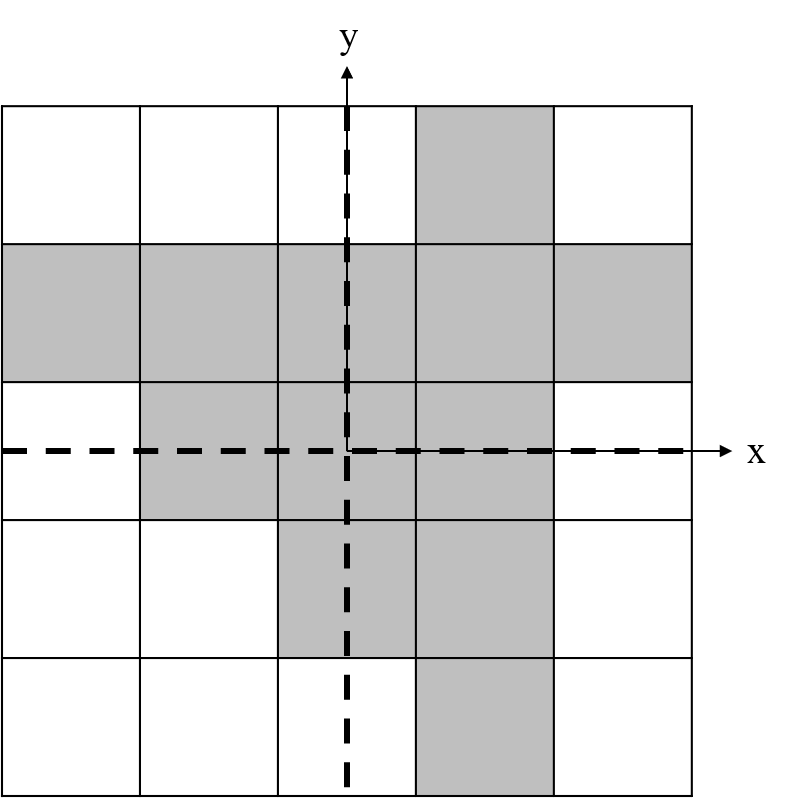
\includegraphics[width=\textwidth]{LSSymRefHV.png}
		\caption{Horizontal and vertical reflection}
	\end{subfigure}
	\hfill
	\begin{subfigure}[t]{0.3\textwidth}
		\centering
		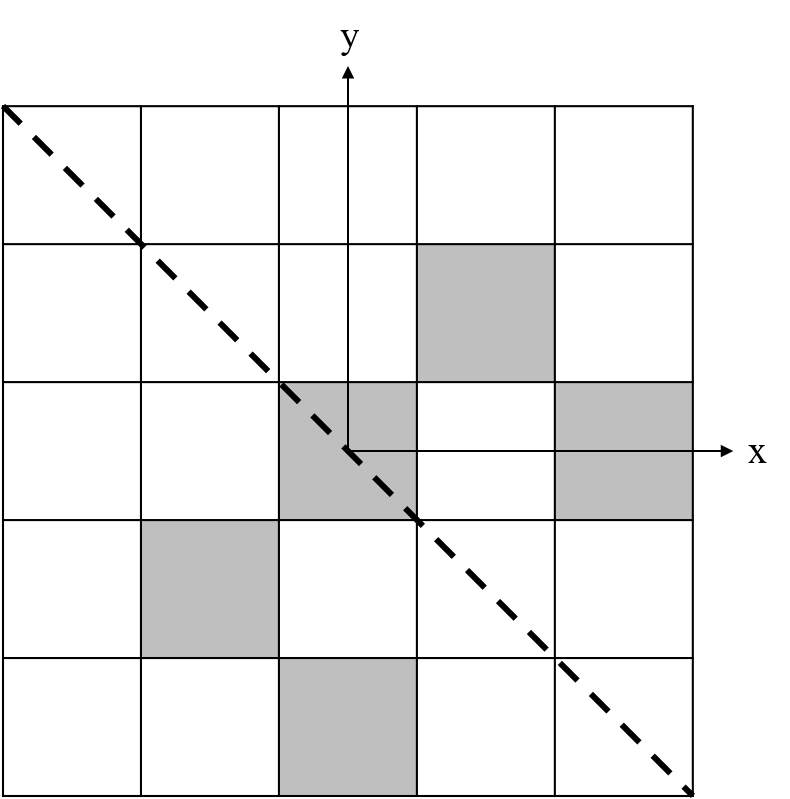
\includegraphics[width=\textwidth]{LSSymRefD.png}
		\caption{Diagonal reflection}
	\end{subfigure}
	\hfill
	\begin{subfigure}[t]{0.3\textwidth}
		\centering
		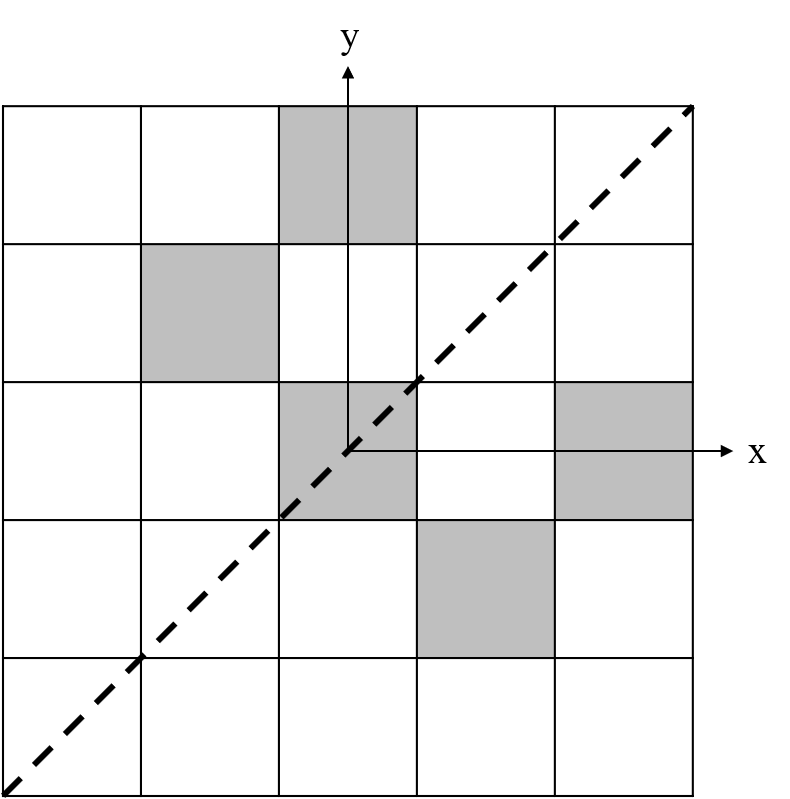
\includegraphics[width=\textwidth]{LSSymRefND.png}
		\caption{Negative diagonal reflection}
	\end{subfigure}
	\hfill
	\begin{subfigure}[t]{0.3\textwidth}
		\centering
		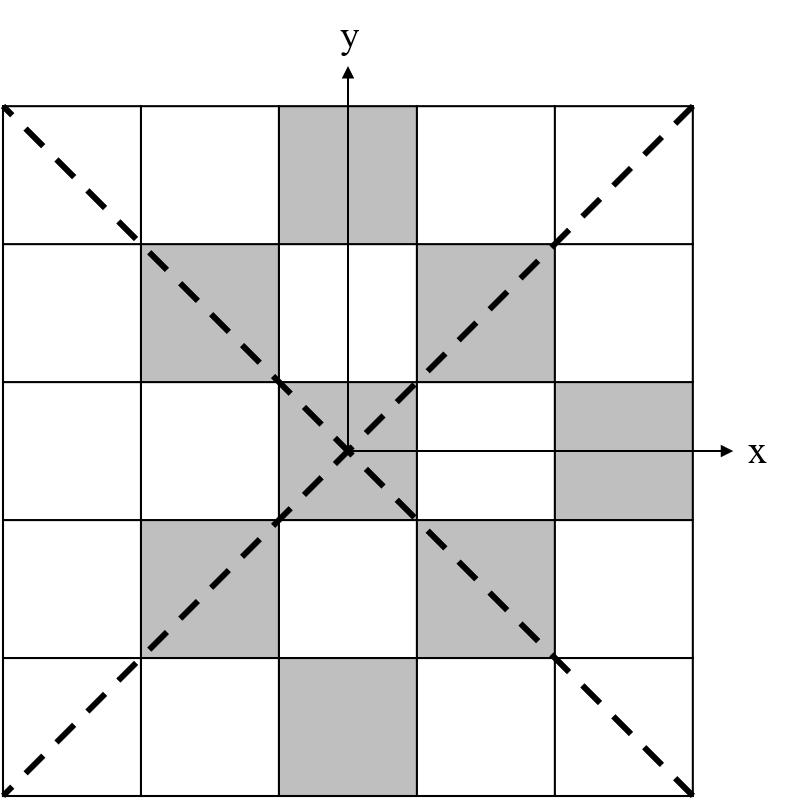
\includegraphics[width=\textwidth]{LSSymRefDND.png}
		\caption{Diagonal and negative diagonal reflection}
	\end{subfigure}
	\caption[L-System symmetry interpretations]{L-System interpretation of symmetry axioms according to Figure~\ref{fig:lssymex}. Axes of symmetry are indicated with dotted lines}
	\label{fig:lssym}
\end{figure}

All L-System rule interpretations are first applied as if the axiom were a single "F". The rules are applied for the specified number of iterations. The resulting word is then placed within the specified axiom of symmetry at all positions occupied by an "F". This allows for the symmetry conditions to be maintained across iterations while retaining "+" and "-" as variables.

\subsubsection{Interpretation}

The final word is interpreted according to the specified internal dimensions of the template. The word is interpreted character by character.

The number of open round brackets in the word is counted. For every open round bracket, the first subsequent closed round bracket is identified. Each string segment starting and ending with an open and closed round bracket is extracted. The round brackets are replaced with the equivalent square brackets. Pluses and minuses are swapped to invert all directional changes within the round brackets. This allows for reflection symmetry conditions to be applied. The original string segment is replaced with the adjusted string segment.

Every character in the word is interpreted from the initial character. The interpretation applies to a grid of squares identified by x- and y-coordinates. The origin square is defined by the coordinates $\left (0,0  \right )$. Positive and negative directions are applied as per standard convention. The interpretation starts at the origin with the direction at \SI{0}{\degree}, i.e. in the positive y-direction.

\begin{figure}[H]
	\centering
	
\includegraphics[width=0.5\textwidth]{LSOrigin.png}
	\caption[L-System origin and orientation]{Example 5x5 grid for L-System interpretation indicating the origin and orientation. The current position is outlined.}
	\label{fig:lso}
\end{figure}

If the character is "F", a check is done to determine if the stack is at its initial value or if the current element is the initial element. If it is either, the element coordinates are set to the origin. If it is neither, the x- and y-coordinates are incremented in the current direction. The new element coordinates are added to the list of coordinates.

If the character is "f", the procedure is identical to the procedure for the character "F", except that the new element coordinates are not added to the list of coordinates. Thus the position is incremented without an element being added.

\begin{figure}[H]
	\centering
	\begin{subfigure}[c]{0.4\textwidth}
		\centering
		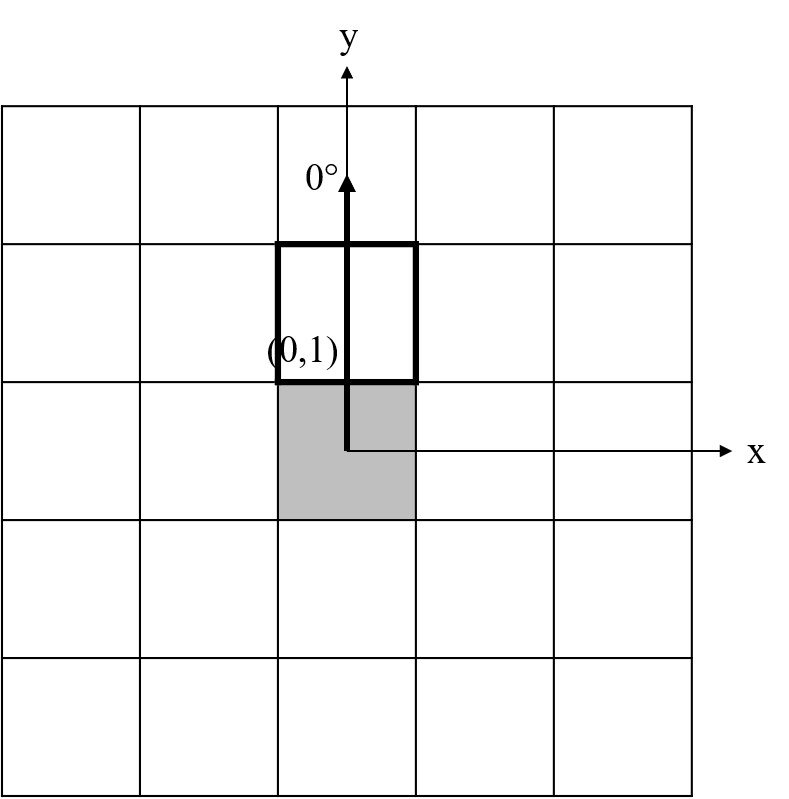
\includegraphics[width=\textwidth]{LSF.png}
		\caption{Interpretation of "F" from the origin. A saved element is filled in.}
	\end{subfigure}
	\hfill
	\begin{subfigure}[c]{0.4\textwidth}
		\centering
		
\includegraphics[width=\textwidth]{LSfsmall.png}
		\caption{Interpretation of "f" from the origin.}
	\end{subfigure}
	\caption[L-System movement interpretation]{L-System interpretation of movement variables}
	\label{fig:lsmove}
\end{figure}

If the character is "+", the current direction is incremented by \SI{45}{\degree}. If the character is "-", the current direction is decremented by \SI{45}{\degree}.

\begin{figure}[H]
	\centering
	\begin{subfigure}[c]{0.4\textwidth}
		\centering
		
\includegraphics[width=\textwidth]{LS+.png}
		\caption{Interpretation of "+" from the origin}
	\end{subfigure}
	\hfill
	\begin{subfigure}[c]{0.4\textwidth}
		\centering
		
\includegraphics[width=\textwidth]{LS-.png}
		\caption{Interpretation of "-" from the origin}
	\end{subfigure}
	\caption[L-System rotation interpretation]{L-System interpretation of rotational variables}
	\label{fig:lsrot}
\end{figure}

If the character is "[", the current position and direction is added to the stack. If the character is "]", a check is done to determine if the stack is at its initial value. If it is, the initial coordinates and direction are fetched. If it is not, the latest coordinates and direction are popped from the stack. A check is then done to determine if the stack is at its initial position. If it is, a flag is set to indicate as such.

The complete list of coordinates is sorted in ascending order. All duplicate element coordinates are removed.

\subsection{CPPNs}
\label{ssec:CPPN}

A CPPN-like generation method is implemented due to the CPPN features of image generation and scalability. CPPNs are defined using class objects containing all necessary information. A single CPPN may generate a number of models. CPPN models are also defined as class objects containing all necessary information.

A random generation seed is used to determine the CPPN's initial layer, hidden layers, and activation functions. The random generation seed allows for replicability of CPPNs.

A CPPN model may be scaled inwards or outwards. The scale parameter was set at 1, i.e. no scaling, in order to reduce complexity. The functionality of the scaling was left implemented to allow for future tests.

The threshold parameter allows for two approaches to the removal of elements. The CPPN outputs 2D arrays of values ranging from 0 to 1. If the threshold parameter is set from 0 to 1, it is interpreted as a rounding threshold. All values above or equal to the threshold are set to 1 and all values below or equal to the threshold are set to 0. If the threshold parameter is set above 1 to 100, it is interpreted as a percentage of elements to remove. The lowest values making up the specified percentage of all values are set to 0 and the rest of the values are set to 1.

The x- and y-dimensions are specified initially. All hidden layers barring the initial layer have a number of nodes equal to the x-dimension multiplied with the y-dimension. The CPPN will result in a model that fits perfectly within the internal space of the unit.

CPPN models obtained for the purposes of this this thesis are at much lower resolutions than traditional CPPN models. A reduction in complexity was deemed appropriate. Traditional CPPNs allow for unique activation functions to be applied to each node. This was not implemented in order to reduce complexity. Five activation functions are available for the hidden layers of the CPPN. Activation functions are applied to an entire layer. The activation functions included in this project are

\begin{itemize}
	\item sin
	\item cos
	\item tanh
	\item sigmoid
	\item smooth ReLu
\end{itemize}

Only the last two activation functions are available for the output layer of the CPPN. They result in values ranging only from 0 to 1. The values are rounded according to the specified threshold parameter.

\section{Generative Design Approaches}
\label{sec:GD}

Generative design methods are required to assist in the determination of well-performing units generated by the pattern generation methods. Large populations of unique units must be created. Each individual's performance should be ranked according to a predefined objective function. Better-performing units should be identified and favoured by the generative design methods.

\subsection{Monte Carlo Simulations}

Monte Carlo simulations operate on the principle that a large enough population of calculated solutions should be fairly representative of the entire population of possible solutions~\citep{Metropolis1949}. A Monte Carlo simulation of units is thus implemented as a generative design method.

A population of units is randomly generated according to the specified unit generation method. The unit generation process is outlined in Section~\ref{ssec:uapg}. The entire unit population is simulated and ranked according to an objective function specified by the template case. The ranking process is discussed in more detail in Section~\ref{ssec:rank}. Further evaluation of unit performance may be carried out by manual inspection of high-ranking units.

\subsection{Evolutionary Algorithms}
\label{ssec:ea}

Evolutionary algorithms involve the initial generation of a random population and the improvement of the population members' fitness according to some objective function over a number of generations. An evolutionary algorithm is thus implemented as a generative design method.

An initial random population is generated, run, and evaluated. Two parent population members are selected for evolution. Parents are ranked in descending order according to their fitness. The ranking procedure is discussed in detail in Section~\ref{ssec:rank}. The parent population is iterated through from the most fit to the least fit parent until a parent has been selected. A random number between 0 and 1 is generated for selection. A fitness weighting function is used to determine the selection of a parent. The fitness weighting function is defined as

\begin{equation}
	y=\frac{2\left ( p+1-r \right )^{c}}{p^{2}+p}
\end{equation}

Where

\begin{itemize}
	\item $y$ is the fitness weighting
	\item $p$ is the population size
	\item $r$ is the rank of the selected member
	\item $c$ is a user-defined fitness constant set to 1
\end{itemize}

The cumulative fitness weighting of all units before and after the current population member is calculated. If the random number is between the two cumulative fitness weightings, the member is selected as the parent. Population members may evolve in three ways.

Crossover may occur between two parents. For every crossover point, a random number between 0 and 1 is generated. If the number is below the specified probability, crossover occurs. A random index in the list of parent parameters is selected. The parameters are swapped between parents from this index onwards. The two resulting children are potentially evolved further.

Random mutation of a child parameter may occur. For every random mutation point, a random number between 0 and 1 is generated. If the number is below the specified probability, random mutation occurs. A random parameter of the child is selected. The parameter is randomly changed to any allowed value for that parameter.

Biased mutation of a child parameter may occur. For every biased mutation point, a random number between 0 and 1 is generated. If the number is below the specified probability, biased mutation occurs. A random parameter of the child is selected. Another random number between 0 and 1 is generated. If the number is below 0.5, the parameter is decreased by 1. If the number is above or equal to 0.5, the parameter is increased by 1. The parameter is bounded by the allowed ranges.

All children are added to the population list. The new population list is used to generate the next population of units.

\section{FEM}

A FEM analysis of material behaviour is implemented. Licensed and maintained FEM software is readily available. As per Section~\ref{sec:SaA}, original FEM code will not be implemented to limit the scope of the project.

\subsection{Template}

The generative design approach as discussed in Section~\ref{sec:GD} requires large populations of similar units to be created and run. The units need to be similar to meaningfully draw comparisons between them and select the best performing units. A template unit is created containing all necessary and non-unique specifications. The template can be altered according to the specified unit generation method.

The template has all appropriate FEM settings applied. The template is a 2D grid of square elements. 2D quad shell elements, each having four nodes, are used. Plane strain geometrical properties are applied to all elements. A single contact body is defined containing all elements. Material properties are added to all elements according to the Ogden material model. Mold Star 15's Ogden material model parameters as per Table~\ref{tab:ogdpar} are applied.

The template has boundary conditions applied causing deformation according to a specified case. Cases are outlined in Section~\ref{sec:UC}. Forced displacement boundary conditions are applied to relevant nodes. Displacement magnitudes are either 0 or a desired magnitude applied according to a table. The table used is defined as a simple $y=x$ function across the interval \SI{0}{\second} to \SI{1}{\second}.

Certain template parameters need to be specified by the user. These parameters are detailed in Section~\ref{ssec:init}. Once the user-specified parameters have been applied, the template may be created. Template creation is described in Section~\ref{ssec:tempcr}.

\subsection{Unit Simulations}
\label{ssec:us}

Units are altered templates. Units have some internal elements removed. It is assumed that units are actuated by an internal pressure. Internal pressures are applied in the FEM models by edge loads perpendicular to all internal edges which have no neighbouring elements. Figure~\ref{fig:uip} illustrates the internal pressure boundary conditions as applied by the software pipeline.

\begin{figure}[H]
	\centering
	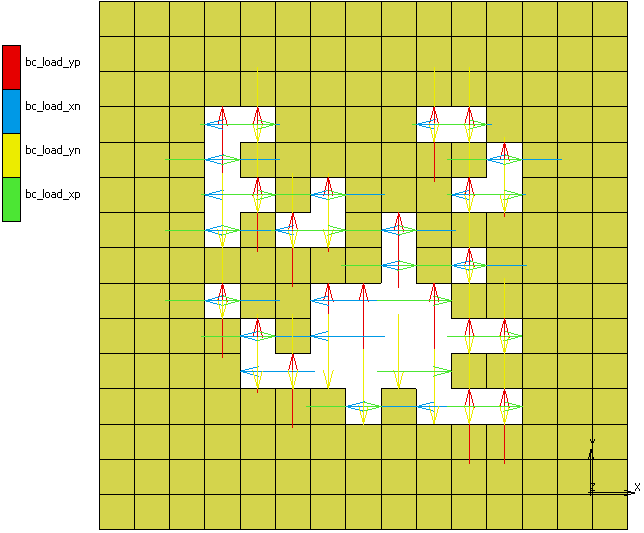
\includegraphics[width=0.5\textwidth]{5x5Single.png}
	\caption[Unit internal pressure boundary conditions]{Unit internal pressure boundary conditions. The unit ID is grid\_39\_1\_973\_1\_8\_28\_42.}
	\label{fig:uip}
\end{figure}

Units are not expected to be utilised independently. It is assumed that multiple units will be arranged together in grid-like patterns to construct actuators with desirable behaviours. Units are thus not modelled in isolation. Units are copied to create a $5\times 5$ grid of identical units. Figure~\ref{fig:5x5grid} illustrates the $5\times 5$ grid created from the unit in Figure~\ref{fig:uip}. Only the central unit is considered during analysis of the results. The central unit is assumed to be representative of a typical unit in a large arrangement.

\begin{figure}[H]
	\centering
	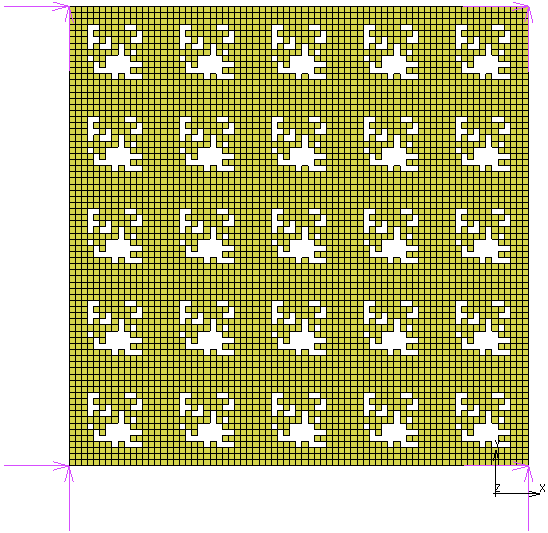
\includegraphics[width=\textwidth]{5x5Layout.png}
	\caption[$5\times 5$ grid layout with fixed boundary conditions indicated]{$5\times 5$ grid layout of the unit in Figure~\ref{fig:uip} with fixed boundary conditions indicated}
	\label{fig:5x5grid}
\end{figure}

Fixed boundary conditions are applied to prevent rigid body modes. The four outermost nodes of the $5\times 5$ grid arrangement are fixed in the x- and y-direction. These boundary conditions are visible in Figure~\ref{fig:5x5grid}.

\section{Unit Deformation Cases}
\label{sec:UC}

Three unit deformation cases were defined, implemented and evaluated with the software pipeline. The pipeline allows for easy implementation of new unit deformation cases and methods of evaluation. The unit deformation cases were selected due to their robustness, potential applications and simplicity.

\subsection{Uniaxial Elongation}

Case 1 is a case of uniaxial elongation as defined by Kim \citep{Kim2015}. This case has no rigid body modes. Four boundary conditions are applied. They are outlined in Table~\ref{tab:c1}.

% Please add the following required packages to your document preamble:
% \usepackage{booktabs}
\begin{table}[H]
\centering
\begin{tabular}{@{}lllc@{}}
\toprule
\multicolumn{1}{c}{\textbf{Label}} & \multicolumn{1}{c}{\textbf{Boundary}} & \multicolumn{1}{c}{\textbf{Constraint}} & \textbf{Direction} \\ \midrule
\textit{bc\_fd\_yy1} & Bottom edge & Fixed               & y \\
\textit{bc\_fd\_yy2} & Top edge    & Forced displacement & y \\
\textit{bc\_fd\_xx1} & Left edge   & Fixed               & x \\
\textit{bc\_fd\_xx2} & Right edge  & Fixed               & x \\ \bottomrule
\end{tabular}
\caption[Uniaxial elongation boundary conditions]{Uniaxial elongation boundary conditions \citep{Kim2015}}
\label{tab:c1}
\end{table}

The boundary conditions as applied in Marc Mentat to a template of $5\times 5$ elements are illustrated in Figure~\ref{fig:c1bc}. The resulting deformation is illustrated in Figure~\ref{fig:c1def}.

\begin{figure}[H]
	\centering
	\begin{subfigure}[b]{0.45\textwidth}
		\centering
		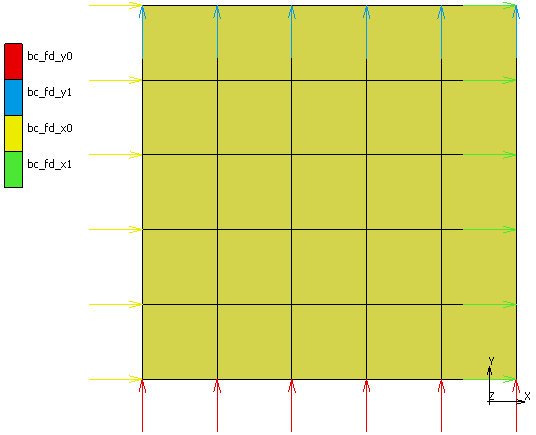
\includegraphics[width=\textwidth]{C1BC.png}
		\caption{Uniaxial elongation boundary conditions as applied in Marc Mentat}
		\label{fig:c1bc}
	\end{subfigure}
	\hfill
	\begin{subfigure}[b]{0.4\textwidth}
		\centering
		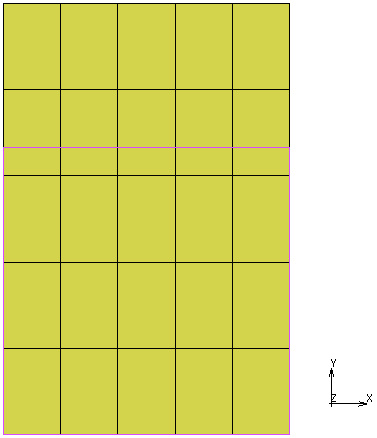
\includegraphics[width=\textwidth]{C1Def.png}
		\caption{Resulting deformation of uniaxial elongation. The original shape is outlined in pink.}
		\label{fig:c1def}
	\end{subfigure}
	\caption[Uniaxial elongation boundary conditions and deformation]{Uniaxial elongation boundary conditions and resulting deformation.}
	\label{fig:c1}
\end{figure}

This case has applications in causing extension. Multiple units combined and oriented in the same direction would result in a linearly extending actuator.

\subsection{Biaxial Elongation}

Case 2 is a case of biaxial elongation. Four boundary conditions are applied. They are outlined in Table~\ref{tab:c2}.

% Please add the following required packages to your document preamble:
% \usepackage{booktabs}
\begin{table}[H]
\centering
\begin{tabular}{@{}lllc@{}}
\toprule
\multicolumn{1}{c}{\textbf{Label}} & \multicolumn{1}{c}{\textbf{Boundary}} & \multicolumn{1}{c}{\textbf{Constraint}} & \textbf{Direction} \\ \midrule
\textit{bc\_fd\_yy1} & Bottom edge & Fixed               & y \\
\textit{bc\_fd\_yy2} & Top edge    & Forced displacement & y \\
\textit{bc\_fd\_xx1} & Left edge   & Fixed               & x \\
\textit{bc\_fd\_xx2} & Right edge  & Forced displacement & x \\ \bottomrule
\end{tabular}
\caption{Biaxial elongation boundary conditions}
\label{tab:c2}
\end{table}

The boundary conditions as applied in Marc Mentat to a template of $5\times 5$ elements are illustrated in Figure~\ref{fig:c2bc}. The boundary conditions are visually identical to Figure~\ref{fig:c1bc}. The resulting deformation is illustrated in Figure~\ref{fig:c2def}.

\begin{figure}[H]
	\centering
	\begin{subfigure}[b]{0.4\textwidth}
		\centering
		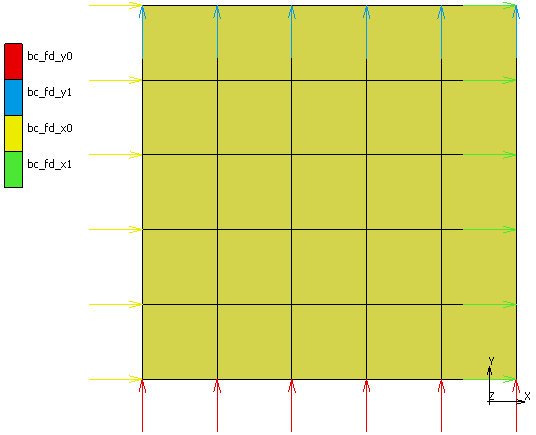
\includegraphics[width=\textwidth]{C1BC.png}
		\caption{Biaxial elongation boundary conditions as applied in Marc Mentat}
		\label{fig:c2bc}
	\end{subfigure}
	\hfill
	\begin{subfigure}[b]{0.45\textwidth}
		\centering
		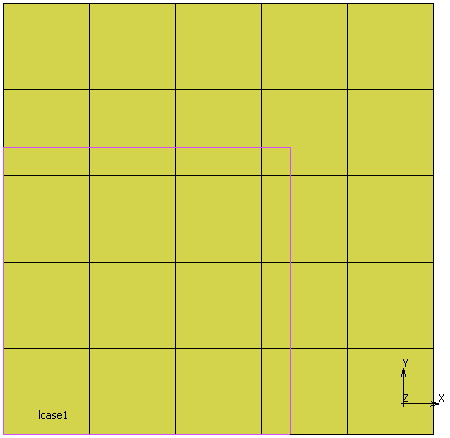
\includegraphics[width=\textwidth]{C2Def.png}
		\caption{Resulting deformation of biaxial elongation}
		\label{fig:c2def}
	\end{subfigure}
	\caption[Biaxial elongation boundary conditions and deformation]{Biaxial elongation boundary conditions and resulting deformation}
	\label{fig:c2}
\end{figure}

This case has applications in causing expansion. Multiple units combined and arranged in a grid would result in an inflating actuator that retains its shape.

\subsection{Pure Shear}

Case 3 is a case of pure shear as defined by Kim \citep{Kim2015}. This case has no rigid body modes. Four boundary conditions are applied. They are outlined in Table~\ref{tab:c3}.

% Please add the following required packages to your document preamble:
% \usepackage{booktabs}
\begin{table}[H]
\centering
\begin{tabular}{@{}lllc@{}}
\toprule
\multicolumn{1}{c}{\textbf{Label}} & \multicolumn{1}{c}{\textbf{Boundary}} & \multicolumn{1}{c}{\textbf{Constraint}} & \textbf{Direction} \\ \midrule
\textit{bc\_fd\_xy1} & Bottom edge & Fixed               & x \\
\textit{bc\_fd\_xy2} & Top edge    & Forced displacement & x \\
\textit{bc\_fd\_yx1} & Left edge   & Fixed               & y \\
\textit{bc\_fd\_yx2} & Right edge  & Fixed				 & y \\ \bottomrule
\end{tabular}
\caption[Pure shear boundary conditions]{Pure shear boundary conditions \citep{Kim2015}}
\label{tab:c3}
\end{table}

The boundary conditions as applied in Marc Mentat to a template of $5\times 5$ elements are illustrated in Figure~\ref{fig:c3bc}. The resulting deformation is illustrated in Figure~\ref{fig:c3def}.

\begin{figure}[H]
	\centering
	\begin{subfigure}[b]{0.4\textwidth}
		\centering
		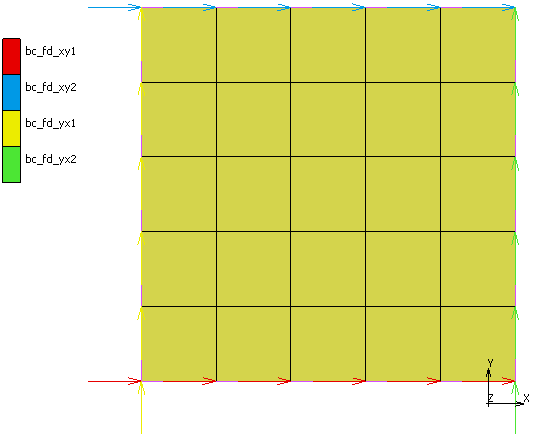
\includegraphics[width=\textwidth]{C3BC.png}
		\caption{Pure shear boundary conditions as applied in Marc Mentat}
		\label{fig:c3bc}
	\end{subfigure}
	\hfill
	\begin{subfigure}[b]{0.45\textwidth}
		\centering
		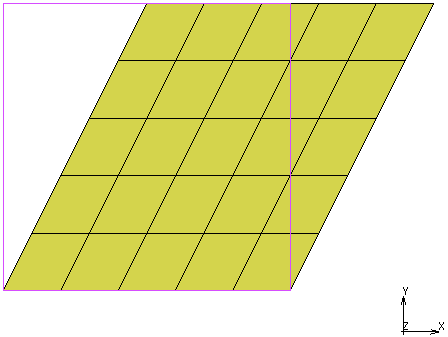
\includegraphics[width=\textwidth]{C3Def.png}
		\caption{Resulting deformation of pure shear}
		\label{fig:c3def}
	\end{subfigure}
	\caption[Pure shear boundary conditions and deformation]{Pure shear boundary conditions and resulting deformation}
	\label{fig:c3}
\end{figure}

This case has applications in causing angular deformation. Multiple units combined and oriented in the same direction would result in an angular actuator. Combining multiple actuators could result in curling actuators or actuators with more complex behaviours.

\subsection{Objective Functions}

To enable the software pipeline to identify well-performing units according to the given template deformation case, objective functions unique to each case must be defined. If cases are added to the software pipeline, objective functions must be added for them as well.

For the uniaxial elongation case, it is desired that the unit elongates while its width remains constant. Two objective functions are identified. The objective function defining elongation is

\begin{equation}
	f=\frac{h}{w}
\end{equation}

Where

\begin{itemize}
	\item $f$ is the objective function value
	\item $h$ is the height of the unit
	\item $w$ is the width of the unit
\end{itemize}

The objective function defining constant width is

\begin{equation}
	f=\max\left (\frac{w}{w_{t}},\frac{w_{t}}{w} \right )
\end{equation}

Where

\begin{itemize}
	\item $w_{t}$ is the width of the template
\end{itemize}

It is desired to maximise both of these functions.

For the biaxial elongation case, it is desired that the unit retains its shape while enlarging. Retaining its shape implies that the height to width ratio remains as close to 1 as possible and that the outer sides remain as straight as possible. Two objective functions are identified. The objective function defining the retention of the height to width ratio is

\begin{equation}
	f=\left | h-w \right |
\end{equation}

The objective function defining the outer sides remaining straight is

\begin{equation}
	f=\sum_{i=1}^{4}H_{d}\left ( s_{t,i},s_{i} \right )
\end{equation}

Where

\begin{itemize}
	\item $s_{t}$ is the set of node coordinates of a side of the template
	\item $s$ is the set of node coordinates of a side of the unit
	\item $H_{d}\left ( x,y \right )$ is the Hausdorff distance as defined in Section~\ref{ssec:Hd}
\end{itemize}

It is desired to minimize both of these functions.

An objective function regarding the enlargement is not defined. The same pressure is applied to all units regardless of the number of elements removed. Units with more elements removed have more edge loads applied. Each edge load is a pressure load of the same magnitude. Elements with more internal edges will have higher total pressures applied and will enlarge more. This would be an unfair objective function compared to the other two selected objective functions. A unit with all internal elements removed may enlarge by a significant factor while another element retains its shape better. The empty unit may rank higher due to a singular high fitness value.

For the pure shear case, it is desired that the top left and right corners shift horizontally to the right with respect to the bottom left and right corners respectively. Three objective functions are identified. The objective functions defining the rightward shift of the top corners are defined as

\begin{equation}
	f=x_{tl}-x_{bl}
\end{equation}

And

\begin{equation}
	f=x_{tr}-x_{br}
\end{equation}

Where

\begin{itemize}
	\item $x_{tl}$ is the x-coordinate of the top left corner
	\item $x_{bl}$ is the x-coordinate of the bottom left corner
	\item $x_{tr}$ is the x-coordinate of the top right corner
	\item $x_{br}$ is the x-coordinate of the bottom right corner
\end{itemize}

The objective function defining constant height is

\begin{equation}
	f=\max\left (\frac{h}{h_{t}},\frac{h_{t}}{h} \right )
\end{equation}

Where

\begin{itemize}
	\item $h_{t}$ is the height of the template
\end{itemize}

It is desired to maximise both of these functions.

\subsubsection{Hausdorff Distance}
\label{ssec:Hd}

\section{Model Validation}
\label{sec:MV}

Validation of the FEM models is preferable in order to verify the accuracy of the experimentally obtained Ogden material model parameters and justify the code pipeline's identification of better-performing units. An experimental setup is designed and constructed to validate the FEM models.

\subsection{Physical Components}
\label{ssec:pc}

A modular mould is designed for the casting of multiple units. Modularity is desirable as all units are derived from a single template, but individual units may vary greatly. Manufacturing times, costs and complexity would be too high if a mould had to be constructed for every unit that was desired to be tested.

The modular mould consists of a mould frame and two types of mould cells. The mould frame is square with dimensions indicated in Figure~\ref{fig:mb}. The cells are square with thicknesses of either \SI{2}{mm} or \SI{4}{mm}, as illustrated in Figure~\ref{fig:mc}. The mould frame is placed on a smooth, level granite tabletop. The mould cells are arranged within the frame according to the layout of the unit to be cast. \SI{2}{mm} cells are placed where elements exist according to the unit layout. \SI{4}{mm} cells are placed where elements have been removed. Figure~ illustrates an example unit layout and the arrangement of the mould before the material has been cast.

\begin{figure}[H]
	\centering
	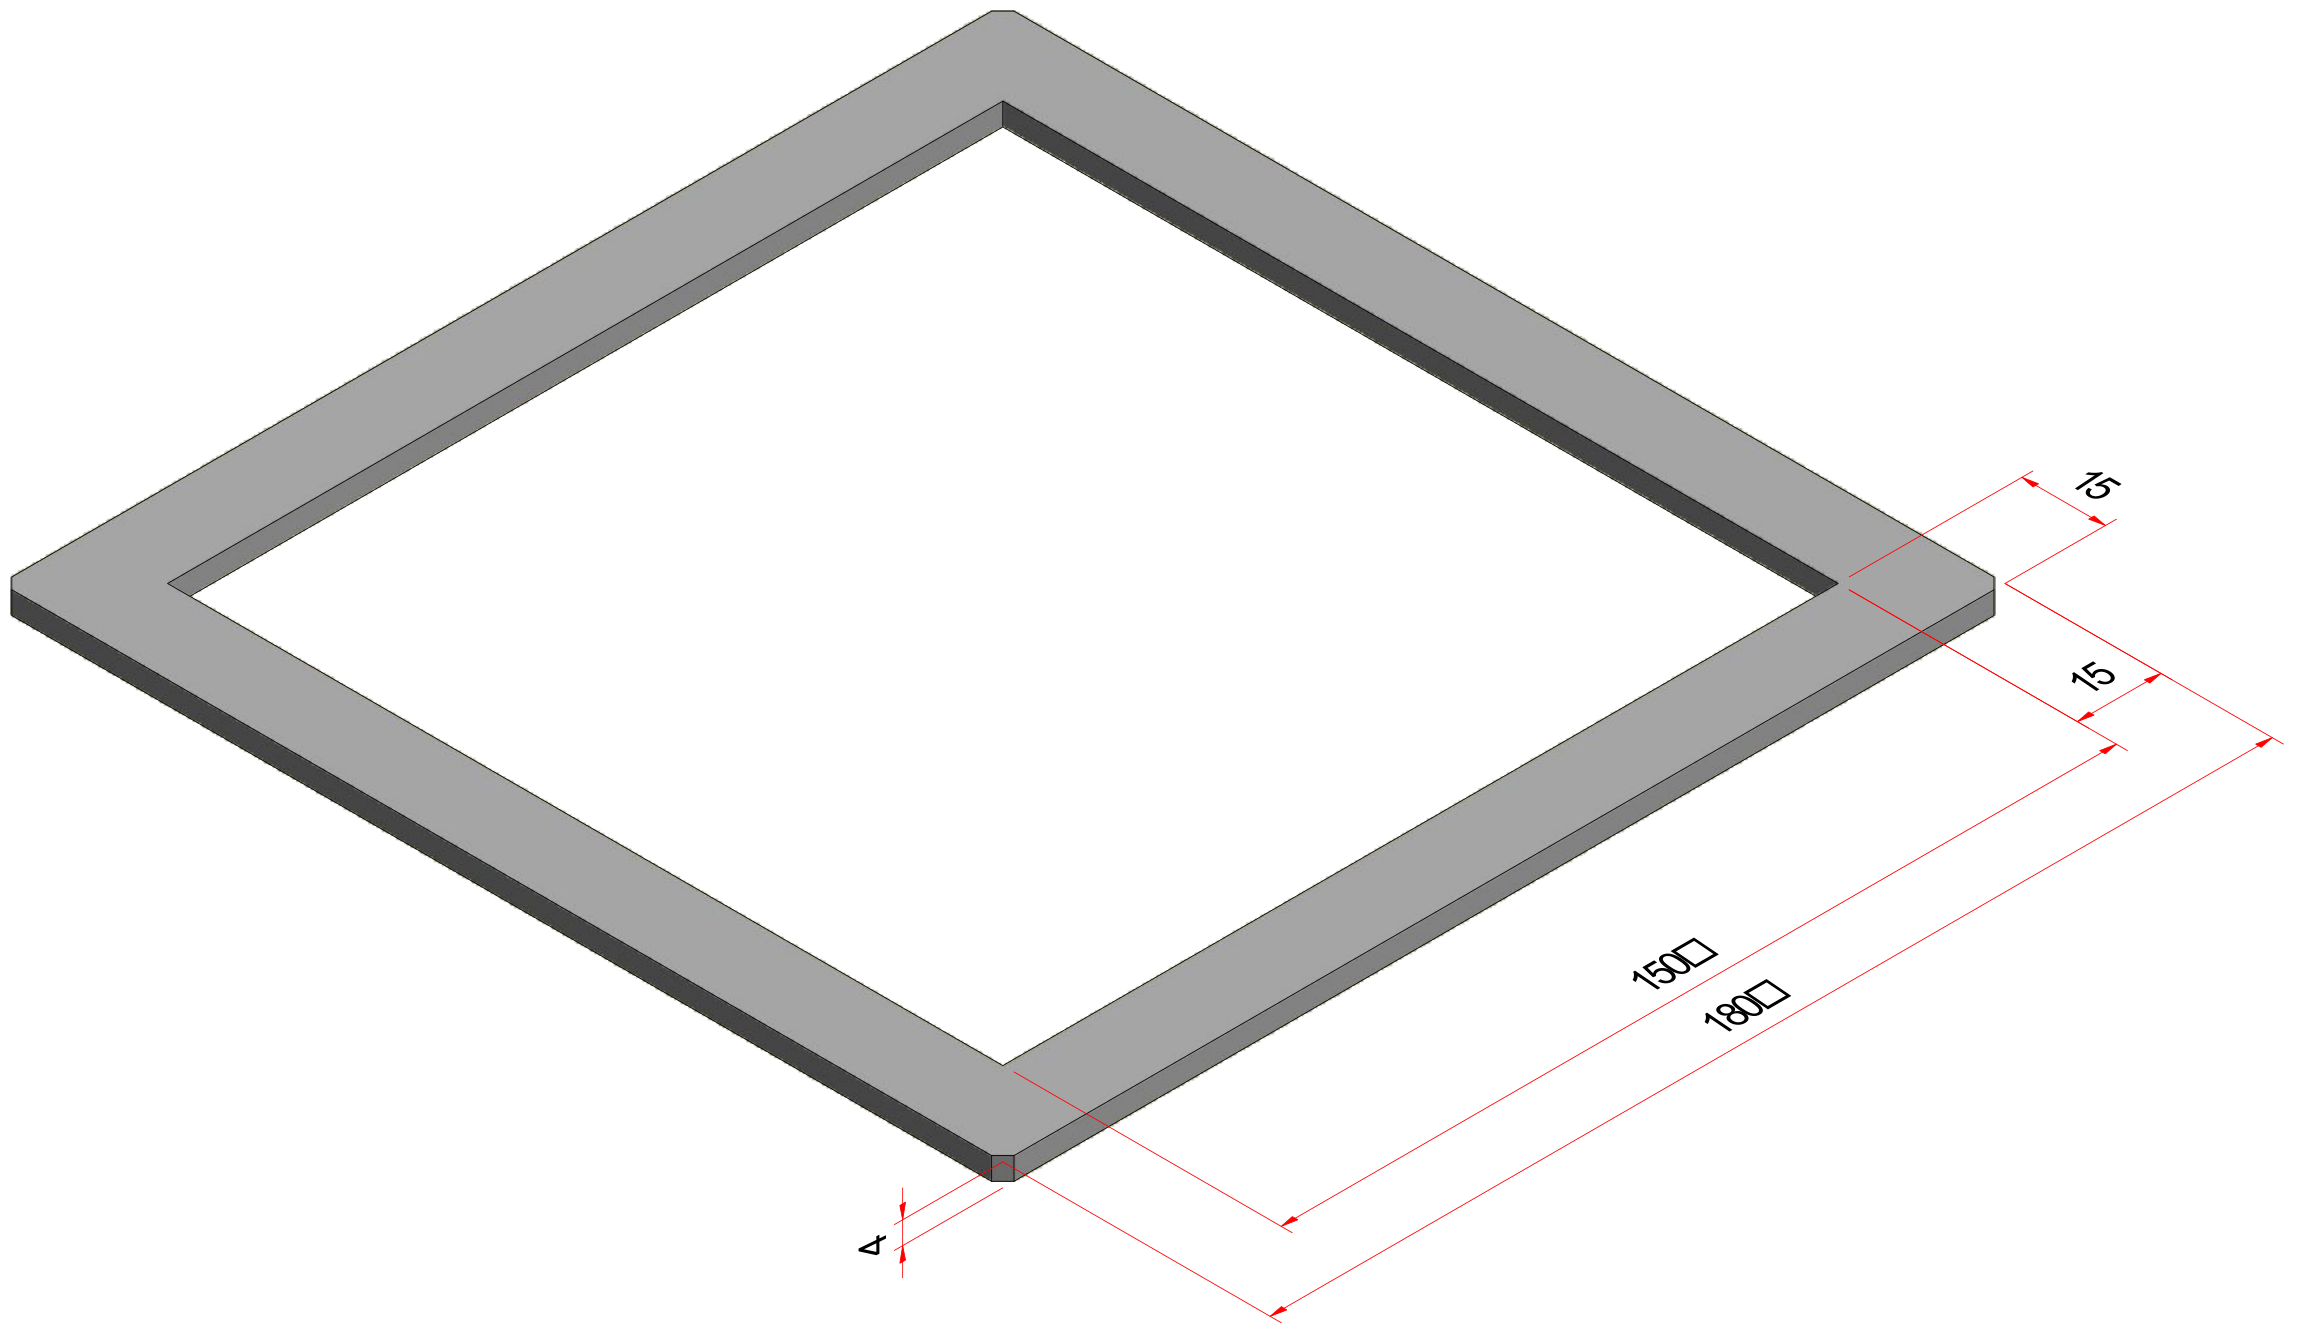
\includegraphics[width=\textwidth]{MB.png}
	\caption{Dimensioned modular mould base}
	\label{fig:mb}
\end{figure}

\begin{figure}[H]
	\centering
	\begin{subfigure}[c]{0.3\textwidth}
		\centering
		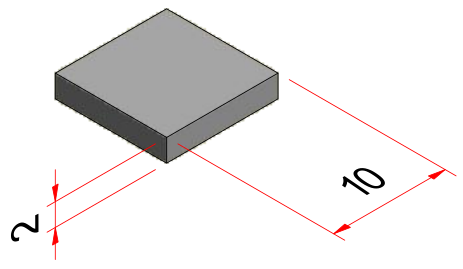
\includegraphics[width=\textwidth]{MCS.png}
		\caption{Small mould cell}
	\end{subfigure}
	\hfill
	\begin{subfigure}[c]{0.3\textwidth}
		\centering
		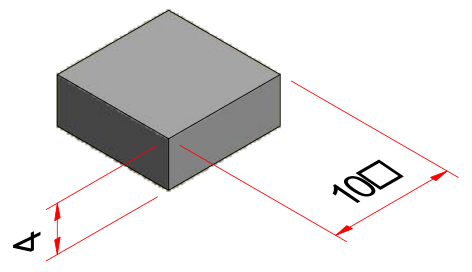
\includegraphics[width=\textwidth]{MCL.png}
		\caption{Large mould cell}
	\end{subfigure}
	\caption{Dimensioned mould cells}
	\label{fig:mc}
\end{figure}

The experimental setup is comprised of two perspex plates separated by 4 \SI{2}{mm} thick washers kept in place by 4 screws, bolts and footpieces on a level surface. The bottom perspex plate has a hole in its centre with a pressure supply tube attached to it. Figure~\ref{fig:exp} illustrates the experimental setup. A camera is affixed to a tripod, positioned over the experimental setup and aimed directly downward at it.

\begin{figure}[H]
	\centering
	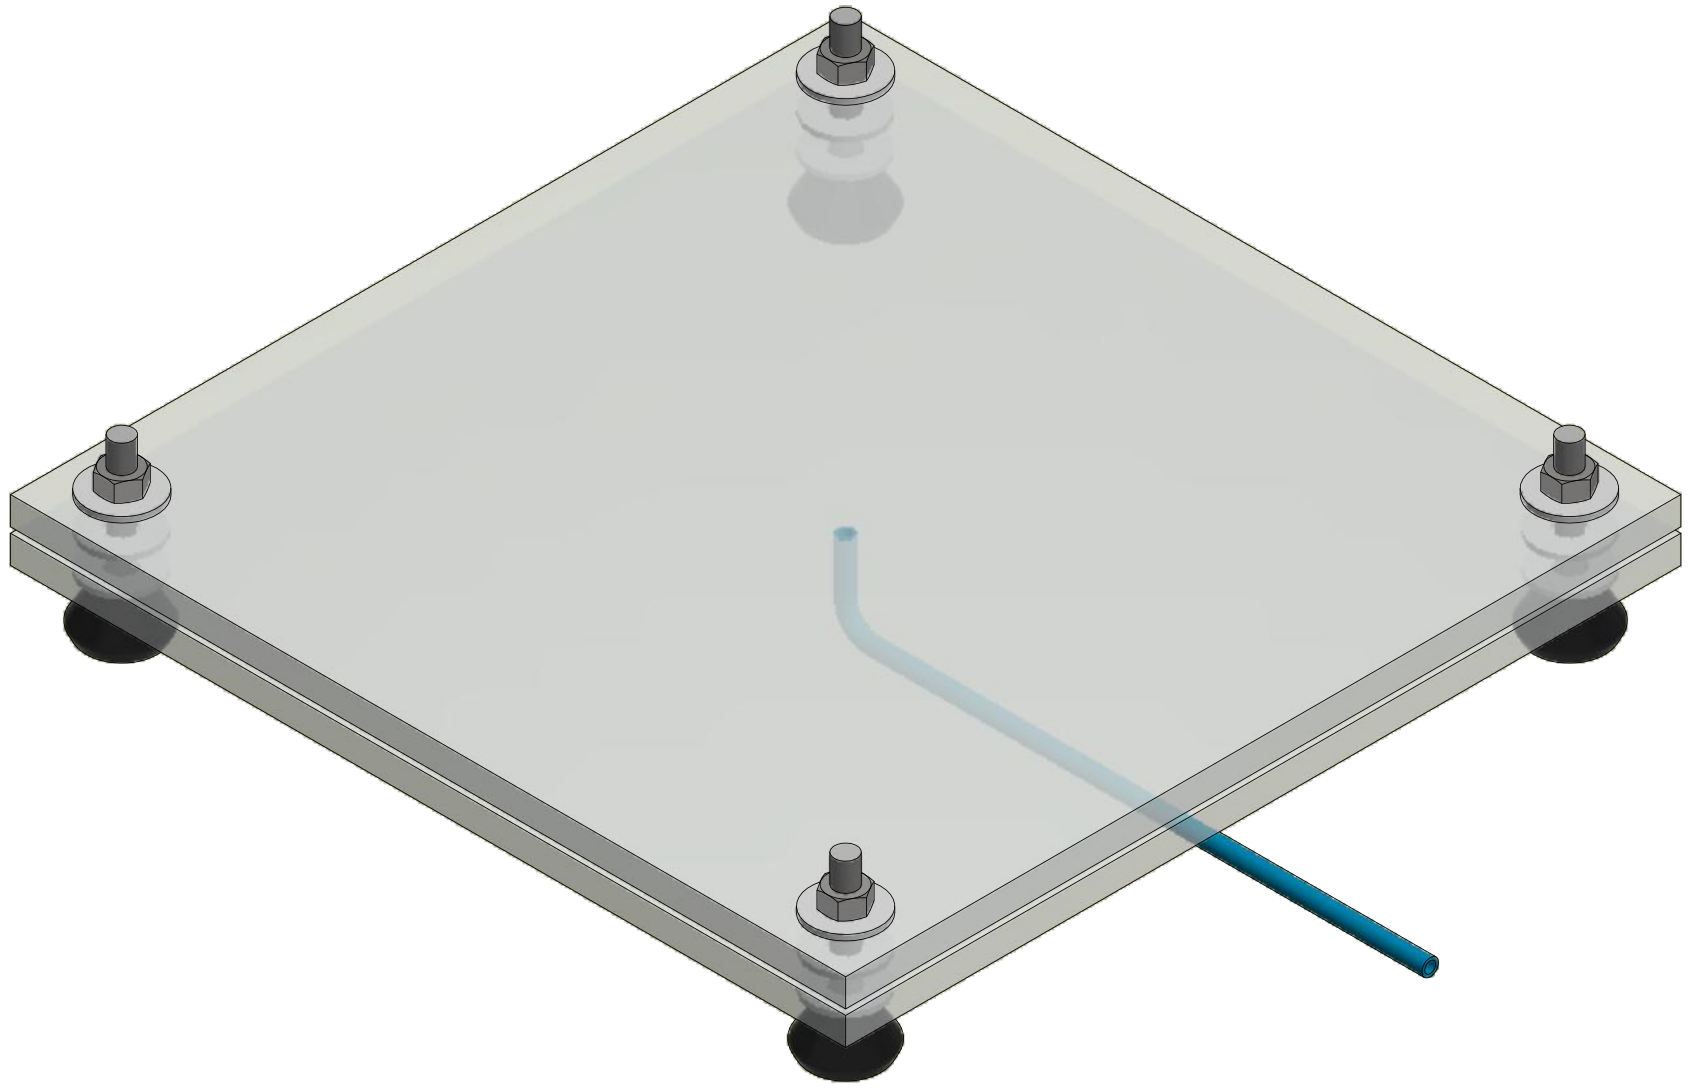
\includegraphics[width=\textwidth]{ER.png}
	\caption{Experimental setup model}
	\label{fig:exp}
\end{figure}

Perspex is selected as the testing surface for various reasons. It has a low frictional coefficient, decreasing the effects of friction on the experiment. It is transparent, allowing for the effects of the applied internal pressure to be viewed and recorded. It is durable enough at the thickness used to resist the internal pressures applied and be manufacturable. It is flexible enough to allow for some deformation without breaking while not deforming due to the internal pressure.

\subsection{Experimental Procedure}
\label{ssec:ep}

The material is cast in the mould after having been prepared as outlined in Section~\ref{ssec:mac}. The physical unit is removed from the mould once it has set completely. The mould may then be rearranged according to a new unit configuration after having been appropriately cleaned.

The FEM models applied a linearly ramping internal pressure to the units. The internal pressure was only applied to a predetermined maximum value. The experimental setup will replicate applied pressures at specific points along the ramp and potentially beyond the maximum simulated pressure.

The experimental setup is put in place with the top perspex plate and bolts having not yet been placed. The surfaces of the perspex plates which will come into contact with the physical unit are lubricated with a silicon-based spray. The spray will react with the physical unit over time, causing it to degrade. Tests must be done in a timely manner to prevent the effects of the spray from impacting results.

The physical unit is placed on the bottom plate with its cavity positioned over the pressure inlet hole. The top plate is affixed to the bottom plate separated by the \SI{2}{mm} washers. The camera is switched on and placed into focus. The pressure valve is slowly opened to desirable pressure intervals. At each interval, photographs are taken of the deformation and the pressure applied is noted.

\section{Software Selection}

The Finite Element Method (FEM) is an approach to numerically solving field problems. Field problems require the determination of one or more dependent variables' distribution in space. Field problems are mathematically described with differential equations or integral expressions. Finite elements can be expressed as small parts of a larger body. A field quantity within an element may only have a simple spatial variation, such as being described by polynomial terms no higher than the second order. FEM differs from calculus as calculus uses infinitesimal elements. FEM thus delivers approximate solutions. \citep{Cook2002}

Several commercial FEM software packages capable of realistically modelling soft bodies are available. LSDyna is a FEM software package widely used in industry. It is owned by ANSYS and maintained by LSTC. The software's code is based on highly non-linear and transient dynamic FEM with explicit time integration \citep{LSDyna}. Siemens NX 12 is an integrated software package capable of performing FEM analysis. The software package has a user-friendly interface for graphical design of components \citep{NX12}. MSC.Marc Mentat is a pre- and postprocessing software for the MSC.Marc FEM solver. It is focused on nonlinear material modelling and analysis. It has an extensive set of options available for post-processing \citep{MSC}.

MSC.Marc Mentat 2019 is selected for this project. Marc Mentat is actively maintained and updated. Tutorials and reference manuals are built into the software. Support is available if issues are encountered or for any other reason. Limitations include the necessity of having continuous access to a license server. An official VPN configuration as well as remote desktop tools allowed for access to the software as long as a network connection could be established.

Python 3.6 is used to construct a modelling pipeline. Packages are available that allow for the integration of Python and Marc. Many advanced numerical analysis packages are also available for Python. The Python code is accessible, installable and editable. Additional information on how to install and edit the code is available in Appendix~.

\section{Software Pipeline}
\label{sec:SW}

The software pipeline is complex, and many components are interrelated. Details considered trivial or irrelevant are not discussed. The entirety of the code is available to the reader if they would wish to investigate or make use of it. The code is extensively commented for any clarification needed.

\subsection{Initialisation}
\label{ssec:init}

Before a set of units is created, the user needs to specify certain parameters for the template, analysis approach and unit generation method.

Template parameters that need to be specified are outlined in Table~\ref{tab:temppar}. Prerequisites for the parameters are included where applicable.

% Please add the following required packages to your document preamble:
% \usepackage{booktabs}
\begin{table}[H]
\centering
\caption[Template class object initial parameters]{Template class object initialisation parameters and prerequisites}
\label{tab:temppar}
\begin{tabular}{@{}llc@{}}
\toprule
\multicolumn{1}{c}{\textbf{Parameter}} & \multicolumn{1}{c}{\textbf{Description}}                                                              & \textbf{Prerequisite} \\ \midrule
\textit{case}                          & The template case identifier                                                                          & 1, 2, 3               \\ \midrule
\textit{x\_e}                          & \begin{tabular}[c]{@{}l@{}}The number of elements in the\\  x-direction\end{tabular}                  & $>0$, int             \\ \midrule
\textit{y\_e}                          & \begin{tabular}[c]{@{}l@{}}The number of elements in the\\  y-direction\end{tabular}                  & $>0$, int             \\ \midrule
\textit{e\_s}                          & \begin{tabular}[c]{@{}l@{}}The side length of the element in\\ \si{mm}\end{tabular}  & $>0$                  \\ \midrule
\textit{b}                             & \begin{tabular}[c]{@{}l@{}}The number of elements reserved\\ for the unit boundary width\end{tabular} & $>0$, int             \\ \midrule
\textit{ogd\_mat} &
  \begin{tabular}[c]{@{}l@{}}The Ogden material model\\ parameters\end{tabular} &
  \textit{\begin{tabular}[c]{@{}c@{}}mold\_star\_15\\ ecoflex\_0030\\ smooth\_sil\_950\end{tabular}} \\ \midrule
\textit{n\_steps} &
  \begin{tabular}[c]{@{}l@{}}The number of analysis steps in\\ \SI{1}{\second} of analysis\end{tabular} &
  $>0$, int \\ \midrule
\textit{table\_name}                   & \begin{tabular}[c]{@{}l@{}}The name of the function applied\\ to the template\end{tabular}            & str                   \\ \midrule
\textit{d\_mag}                        & The applied displacement in \si{mm}                                                  &                       \\ \midrule
\textit{p\_mag}                        & \begin{tabular}[c]{@{}l@{}}The applied internal pressure in\\ \si{MPa}\end{tabular}  &                       \\ \bottomrule
\end{tabular}
\end{table}

The template case identifier refers to the unit deformation cases in order as outlined in Section~\ref{sec:UC}. Additional unit deformation cases may be defined by adding the appropriate code, as well as additional Ogden material models.

A unit boundary is always included. The unit boundary is a layer of elements along the side of the unit which are not allowed to be removed by the unit generation process. The unit boundary ensures that the internal geometry remains enclosed to allow for inflation. The unit boundary also ensures that units will always be capable of being packed into a grid alongside one another.

The name of the function applied to the template is a simple string label to identify the graph type applied to the deformation and internal pressure boundary conditions. The graph may be modified from the currently implemented ramp input to any graphical function by editing the Python code appropriately.

Analysis approach parameters that need to be specified are outlined in Table~\ref{tab:analpar}. Prerequisites for the parameters are included where applicable.

% Please add the following required packages to your document preamble:
% \usepackage{booktabs}
\begin{table}[H]
\centering
\caption{Analysis approach initialisation parameters and prerequisites}
\label{tab:analpar}
\begin{tabular}{@{}llc@{}}
\toprule
\textit{\textbf{Parameter}} & \textit{\textbf{Description}} & \multicolumn{1}{l}{\textit{\textbf{Prerequisite}}} \\ \midrule
\textit{a\_meth} & The analysis approach method    & m, g      \\
\textit{g\_meth} & The unit generation method      & r, l, c   \\
\textit{n\_u}    & The number of units to generate & $>0$, int \\ \bottomrule
\end{tabular}
\end{table}

The analysis approach method is specified by a single character. An "m" indicates the Monte Carlo method should be used. A "g" indicates the evolutionary algorithm method should be used. The unit generation method is specified by a single character. An "r" indicates random unit generation should be used. An "l" indicates L-Systems should be used. A "c" indicates CPPNs should be used. Additional analysis approach methods and unit generation methods may be defined by adding the appropriate code.

The number of units to generate applies to the entire Monte Carlo method, or a single generation's population if the evolutionary algorithm is used.

\subsection{Template Creation}
\label{ssec:tempcr}

The user-specified template parameters are used to define a template class object. The template class object calculates more parameters used in the construction of the template. The relevant calculated parameters are outlined in Table~\ref{tab:tempcalcpar}.

% Please add the following required packages to your document preamble:
% \usepackage{booktabs}
\begin{table}[H]
\centering
\caption[Template class object calculated parameters]{Template class object internally calculated parameters}
\label{tab:tempcalcpar}
\begin{tabular}{@{}lll@{}}
\toprule
\multicolumn{1}{c}{\textbf{Variable}} &
  \multicolumn{1}{c}{\textbf{Description}} &
  \textbackslash{}textbf\{Formula\} \\ \midrule
\textit{x\_s} &
  \begin{tabular}[c]{@{}l@{}}The side length of the template\\ in \si{mm} in the x-direction\end{tabular} &
  \multicolumn{1}{c}{$e\_s\times x\_e$} \\ \midrule
\textit{y\_s} &
  \begin{tabular}[c]{@{}l@{}}The side length of the template\\ in \si{mm} in the y-direction\end{tabular} &
  \multicolumn{1}{c}{$e\_s\times y\_e$} \\ \midrule
\textit{x\_n} &
  \begin{tabular}[c]{@{}l@{}}The number of nodes in the\\ x-direction\end{tabular} &
  \multicolumn{1}{c}{$x\_e+1$} \\ \midrule
\textit{y\_n} &
  \begin{tabular}[c]{@{}l@{}}The number of nodes in the\\ y-direction\end{tabular} &
  \multicolumn{1}{c}{$y\_e+1$} \\ \midrule
\textit{n\_e} &
  \begin{tabular}[c]{@{}l@{}}The total number of elements\\ in the template\end{tabular} &
  \multicolumn{1}{c}{$x\_e\times y\_e$} \\ \midrule
\textit{n\_n} &
  \begin{tabular}[c]{@{}l@{}}The total number of nodes in\\ the template\end{tabular} &
  \multicolumn{1}{c}{$x\_n\times y\_n$} \\ \midrule
\textit{e\_internal} &
  \begin{tabular}[c]{@{}l@{}}The list of internal element IDs\\ that are allowed to be removed\end{tabular} &
  Function \\ \midrule
\textit{n\_external} &
  The list of external node IDs &
  Function \\ \midrule
\textit{t\_id} &
  The template ID &
  Function \\ \midrule
\textit{grid} &
  A representative grid of ones &
  Function \\ \midrule
\textit{fp\_t} &
  The file paths of all relevant files &
  Function \\ \bottomrule
\end{tabular}
\end{table}

The list of internal element IDs refers to the elements contained within the boundary of the unit. Only these elements are allowed to be removed by the unit generation method. The IDs are obtained by an internal function. The function algorithm is detailed in Figure~.

The template ID is a formatted string. The ID is generated using unique template class object parameters. The ID is formatted as

\vspace{\baselineskip}

\centerline{grid\_<\textit{case}>\_<\textit{x\_e}>x<\textit{y\_e}>\_<\textit{x\_s}>x<\textit{y\_s}>}

\vspace{\baselineskip}

A grid of ones is generated to represent the template in coordinate calculations. The grid is generated according to the element resolution of the template. Ones are representative of elements in place. When elements are removed during unit generation, they are replaced with zeroes.

The file paths are generated for all relevant files. The template ID is used as the base name of every file. Additional identifiers and file formats are appended as necessary. A more detailed description of the file management system may be found in Section~.

The template is created in Marc Mentat. The nodes are created starting at the global origin on the XY-plane. The nodes are incrementally added in the positive x-direction. The nodes are spaced apart as defined by \textit{e\_s}. Once a row of nodes is completed as defined by \textit{x\_n}, the y-coordinate is positively incremented as defined by \textit{e\_s}. A new row of nodes is created. This process is repeated until completed as defined by \textit{y\_n}.

Four nodes are used to make square 2D elements. Starting at the global origin, elements are incrementally added in the x-direction until completed as defined by \textit{x\_e}. All rows are added until completed as defined by \textit{y\_e}.

The graph used to apply the boundary conditions is defined. The boundary conditions are applied according to the case identifier. The boundary conditions related to each case are detailed in Section~\ref{sec:UC}.

Mechanical planar strain geometric properties are added to all elements. The Ogden material model for Mold-Star 15 is applied to all elements. A single contact body is defined containing all elements. The loadcase containing the fixed and forced displacement boundary conditions is created. The job for the loadcase is created.

The template is saved at this point. All units created during a simulation are built from this template. The template job is run and its success evaluated. The process of running a simulation and evaluating its success is outlined in Section~\ref{ssec:run}.

The template model is saved again. Meaningful template parameters and data obtained from the template is written in a human-readable manner to a log file. The template class object is saved to a file that can be accessed later.

\subsection{Unit and Population Generation}
\label{ssec:uapg}

Unit generation refers to the process of automatically generating internal geometry of a unit based on the predefined template. Three methods of unit generation are implemented and investigated. All three methods provide a list of internal element IDs provided to MarcMentat as elements to be removed from the template file.

Random generation is implemented as a baseline to compare with the other two unit generation methods. A random generation seed is used to allow for replicability. A number of elements to be removed is first selected. A list of unique internal element IDs is then selected and sorted.

L-Systems and CPPNs as outlined in Sections~\ref{ssec:LS} and~\ref{ssec:CPPN} respectively are also available for unit generation. A list of maximum and minimum parameter values is defined. The parameter values are appropriate to the unit generation method specified. The different parameters, ranges and motivations are outlined in Table~\ref{tab:ungenmethpar}. The range values are inclusive.

% Please add the following required packages to your document preamble:
% \usepackage{booktabs}
% \usepackage{multirow}
% \usepackage{graphicx}
\begin{table}[H]
\centering
\resizebox{\textwidth}{!}{%
\begin{tabular}{@{}lccl@{}}
\toprule
\multicolumn{1}{c}{\multirow{2}{*}{\textbf{Parameter}}} &
  \multicolumn{2}{c}{\textbf{Range}} &
  \multicolumn{1}{c}{\multirow{2}{*}{\textbf{Motivation}}} \\ \cmidrule(lr){2-3}
\multicolumn{1}{c}{} &
  \textbf{Min} &
  \textbf{Max} &
  \multicolumn{1}{c}{} \\ \midrule
\multicolumn{4}{c}{\textbf{Random}} \\ \midrule
Seed &
  1 &
  \begin{tabular}[c]{@{}c@{}}Number of units\\ to be generated\end{tabular} &
  \begin{tabular}[c]{@{}l@{}}The seed is limited to the number of\\ units requested by the simulation\end{tabular} \\
\begin{tabular}[c]{@{}l@{}}Number of \\ elements removed\end{tabular} &
  0 &
  \begin{tabular}[c]{@{}c@{}}Number of\\ internal elements\end{tabular} &
  \begin{tabular}[c]{@{}l@{}}The complete range of elements which\\ may potentially be removed is included\end{tabular} \\ \midrule
\multicolumn{4}{c}{\textbf{L-System}} \\ \midrule
Seed &
  1 &
  \begin{tabular}[c]{@{}c@{}}Number of units\\ to be generated\end{tabular} &
  \begin{tabular}[c]{@{}l@{}}The seed is limited to the number of\\ units requested by the simulation\end{tabular} \\
Axiom ID &
  1 &
  \begin{tabular}[c]{@{}c@{}}Number of\\ predefined axioms\end{tabular} &
  The complete list of axioms is included \\
Number of rules &
  1 &
  \begin{tabular}[c]{@{}c@{}}Number of\\ L-System variables\end{tabular} &
  \begin{tabular}[c]{@{}l@{}}At least one rule is required for a valid\\ L-System, and the number of rules is\\ limited to the number of L-System variables\end{tabular} \\
Rule length &
  2 &
  5 &
  \begin{tabular}[c]{@{}l@{}}A rule must be longer than one character,\\ and potential complexity is limited\end{tabular} \\
\begin{tabular}[c]{@{}l@{}}Number of\\ iterations\end{tabular} &
  1 &
  5 &
  \begin{tabular}[c]{@{}l@{}}At least one iteration must be applied for a\\ valid L-System, and potential complexity is\\ limited\end{tabular} \\ \midrule
\multicolumn{4}{c}{\textbf{CPPN}} \\ \midrule
Seed &
  1 &
  \begin{tabular}[c]{@{}c@{}}Number of units\\ to be generated\end{tabular} &
  \begin{tabular}[c]{@{}l@{}}The seed is limited to the number of units\\ requested by the simulation\end{tabular} \\
Model ID &
  1 &
  N/A &
  Potential complexity is limited \\
Scale &
  1 &
  N/A &
  Potential complexity is limited \\
\begin{tabular}[c]{@{}l@{}}Number of\\ hidden layers\end{tabular} &
  2 &
  10 &
  \begin{tabular}[c]{@{}l@{}}At least two layers are required to have a\\ valid network, and potential complexity is\\ limited\end{tabular} \\
\begin{tabular}[c]{@{}l@{}}Size of the initial\\ hidden layer\end{tabular} &
  2 &
  32 &
   \\
\begin{tabular}[c]{@{}l@{}}Element removal\\ threshold\end{tabular} &
  0 &
  100 &
  \begin{tabular}[c]{@{}l@{}}The complete range of elements which\\ may potentially be removed is included\end{tabular} \\ \bottomrule
\end{tabular}%
}
\caption[Unit generation method parameter ranges]{Unit generation method parameter ranges and motivations}
\label{tab:ungenmethpar}
\end{table}

A population of units is generated according to the specified unit generation method. Each population member is a list of parameters within the bounds specified in Table~\ref{tab:ungenmethpar}. If the unit generation method is random, the two parameters are used to generate a list of elements to be removed directly.

If the unit generation method is specified as L-Systems, the parameters are used to generate a random L-System class object. Specified and internally generated L-System class object parameters are outlined in Table~\ref{tab:lspardes}.

% Please add the following required packages to your document preamble:
% \usepackage{booktabs}
\begin{table}[H]
\centering
\caption{L-System class object parameters and descriptions}
\label{tab:lspardes}
\begin{tabular}{@{}ll@{}}
\toprule
\multicolumn{1}{c}{\textbf{Parameter}} & \multicolumn{1}{c}{\textbf{Description}}                 \\ \midrule
\textit{seed}                          & The random generation seed used to generate the L-System \\
\textit{vocab}                         & The L-System vocabulary                                  \\
\textit{gramm}                         & The L-System grammar                                     \\
\textit{axiom}                         & The initial axiom of the L-System                        \\
\textit{n}                             & The number of iterations to apply to the L-System        \\
\textit{word}                          & The resulting word of the L-System                       \\ \bottomrule
\end{tabular}
\end{table}

The L-System word is interpreted to obtain a list of elements to be removed. L-System word characters are interpreted according to Tables~\ref{tab:lsvarint} and~\ref{tab:lsconint}. The interpretation is done from the first character in the word to the last. The interpretation results in a set of coordinates centred around $\left (0,0  \right )$. The coordinates are shifted from being centred around the origin to being centred around the central element of the unit. All coordinates outside of the internal space of the unit are dropped. The remaining coordinates are interpreted as element indices. These element indices are compared to the list of all internal element indices to obtain the list of elements to be removed.

If the unit generation method is specified as CPPNs, the parameters are used to generate a random CPPN class object. Relevant CPPN class object parameters are outlined in Table~\ref{tab:cppardes}. The CPPN is set to generate the maximum number of models specified by the parameter. A CPPN model class object is defined with the model ID specified by the current parameters. CPPN model class object parameters are outlined in Table~\ref{tab:cpmodpardes}.

% Please add the following required packages to your document preamble:
% \usepackage{booktabs}
\begin{table}[H]
\centering
\caption{CPPN class object parameters and descriptions}
\label{tab:cppardes}
\begin{tabular}{@{}ll@{}}
\toprule
\multicolumn{1}{c}{\textbf{Parameter}} & \multicolumn{1}{c}{\textbf{Description}}             \\ \midrule
\textit{seed}                          & The random generation seed used to generate the CPPN \\
\textit{mod\_n}                        & The number of models to be generated by the CPPN     \\
\textit{scale}                         & The scale of the focus on the model                  \\
\textit{hl\_n}                         & The number of hidden layers in the network           \\
\textit{hl\_s}                         & The size of the initial hidden layer                 \\
\textit{thresh}                        & The rounding or element removal threshold            \\
\textit{x}                             & The number of elements in the x-direction            \\
\textit{y}                             & The number of elements in the y-direction            \\
\textit{res}                           & The resolution of the resulting models               \\
\textit{grid}                          & The resulting models                                 \\ \bottomrule
\end{tabular}
\end{table}

% Please add the following required packages to your document preamble:
% \usepackage{booktabs}
\begin{table}[H]
\centering
\caption{CPPN model class object parameters and descriptions}
\label{tab:cpmodpardes}
\begin{tabular}{@{}ll@{}}
\toprule
\multicolumn{1}{c}{\textbf{Parameter}} & \multicolumn{1}{c}{\textbf{Description}}            \\ \midrule
\textit{cppn}                          & The CPPN class object containing all defined models \\
\textit{mod\_id}                       & The ID of the CPPN model                            \\
\textit{grid}                          & The binary model                                    \\ \bottomrule
\end{tabular}
\end{table}

The resulting grid from the CPPN model class object is a binary 2D grid dimensioned according to the internal space from which elements may be removed. The binary 2D grid is interpreted to obtain element indices for every zero. This list of element indices is the list of elements to be removed.

Each list of elements to be removed is paired with its unit generation method class object or list of parameters. Each pair is added to the population list. For each population member, the template is opened and the relevant elements are removed. Further settings are applied as outlined in Section~\ref{ssec:us}.

It was observed during initial testing that many units generated with L-Systems had either all or no internal elements removed. Two units, one with all elements removed and one with no elements removed, are generated and evaluated before a population is generated. If any population member is detected to have all or no internal elements removed, it is not evaluated again. Results from the relevant initial units generated are attributed to it. This reduces the overall runtime of the simulations.

\subsection{Running a Job}
\label{ssec:run}

The command to run the job is sent to Marc Mentat. Jobs may take anywhere from \SI{0.01}{\second} to \SI{300}{\second} to complete. This depends on the complexity of the model and the number of cut-backs during calculation required to accurately solve for the model behaviour.

Marc Mentat creates several files during the process of running a job. The log file specifies the exit condition of the job. The log file is not created at the start of the job.

A model is always saved just before a job is run. The time stamp of this saved model is used for evaluation of the log file. It is first determined if the log file exists. If it does not exist, the code waits for 1 second before checking again. This repeats until the log file is found to exist. If the log file is found, its time stamp is compared to the model file's time stamp. If the log file is older than the model, i.e. it is a log file of a previous run of the model, the code waits 1 second before checking if it has been updated. If the log file is newer than the model, it is inspected for the exit number string or the access violation string.

If the exit number string is found, the exit number is evaluated. Two exit numbers and an error case are identified and defined in Table~\ref{tab:exno}.

% Please add the following required packages to your document preamble:
% \usepackage{booktabs}
% \usepackage[normalem]{ulem}
% \useunder{\uline}{\ul}{}
\begin{table}[H]
\centering
\begin{tabular}{@{}cl@{}}
\toprule
\textbf{Exit Number} & \multicolumn{1}{c}{\textbf{Description}}       \\ \midrule
3004                 & A successful run                               \\
67                   & A license server connection timeout or failure \\
Other                & An unsuccessful run                            \\ \bottomrule
\end{tabular}
\caption{Marc Mentat exit number descriptions}
\label{tab:exno}
\end{table}

If exit number 3004 is found, the model is recognized as having run successfully. The model output file is opened. All relevant data is read from the model output file and written to clearly labeled CSV files. Any relevant data that must be calculated externally from Marc Mentat is calculated and also written to clearly labeled CSV files. Relevant data is outlined and motivated in Section .

If exit number 67 is found, the job is rerun and the entire process as detailed above is repeated until the exit number can be rerun again. If an access violation string is found, it is treated identically to exit number 67.

If any other exit number is found, an error message with the number is displayed. No results are obtained from the model. The model ID is logged appropriately.

The model is saved and the template model is reopened. The code continues on to the next model.

\subsection{Analysis Approach}
\label{ssec:aa}

If the analysis approach was specified as the Monte Carlo method, a single population of units is generated and ranked. Further evaluation of unit performance may be carried out by manual inspection.

If the analysis approach was specified as evolutionary algorithms, multiple populations of units are generated, ranked, and evolved using the evolutionary algorithm outlined in Section~\ref{ssec:ea}.

\subsection{Ranking}
\label{ssec:rank}

Unit objective function evaluations, or performance measures, are weighted equally. To compare performance measures equivalently, values are studentized according to

\begin{equation}
	f=\frac{x-mean}{std}
\end{equation}

Where

\begin{itemize}
	\item $f$ is the fitness value
	\item $x$ is the performance measure
	\item $mean$ is the mean of all units' performance measures
	\item $std$ is the standard deviation of all units' performance measures
\end{itemize}

All fitness values applicable to a unit are summed together. Units are ranked in either descending or ascending order, depending on whether objective functions were desired to be maximised or minimised respectively.

A list of the ranked population members is generated. All empty or full units are inserted in the list at the position occupied by the initially generated empty or full units. All failed units are appended to the end of the list.

\subsection{File Management}
\label{ssec:fm}

A massive amount of FEM and log files are generated by the software pipeline. A single successful FEM model simulation results in five files being generated by Marc Mentat. An additional log file is generated by the Python code. Thousands of units may be generated during a simulation. Multiple log and graph files are generated for every population.

File names and paths are necessarily generated by the Python code. A hierarchical file naming system was set up to generate unique file names and paths. The file naming system efficiently sorts files according to the template parameters, unit parameters, and time of the simulation. The file naming system generates unique names for every unit generated based on the unit parameters. Files are easily sorted through manually by a user looking to inspect a specific unit, or by the code attempting to access it. Desired alterations to the default file path need only be made once because of the hierarchical nature of the system and the implemented code methodology.

Figure~\ref{fig:fh} illustrates the file hierarchy. Parameters are outlined in Table~\ref{tab:fhpar}.

\begin{landscape}
 \begin{figure}[H]
  \centering
  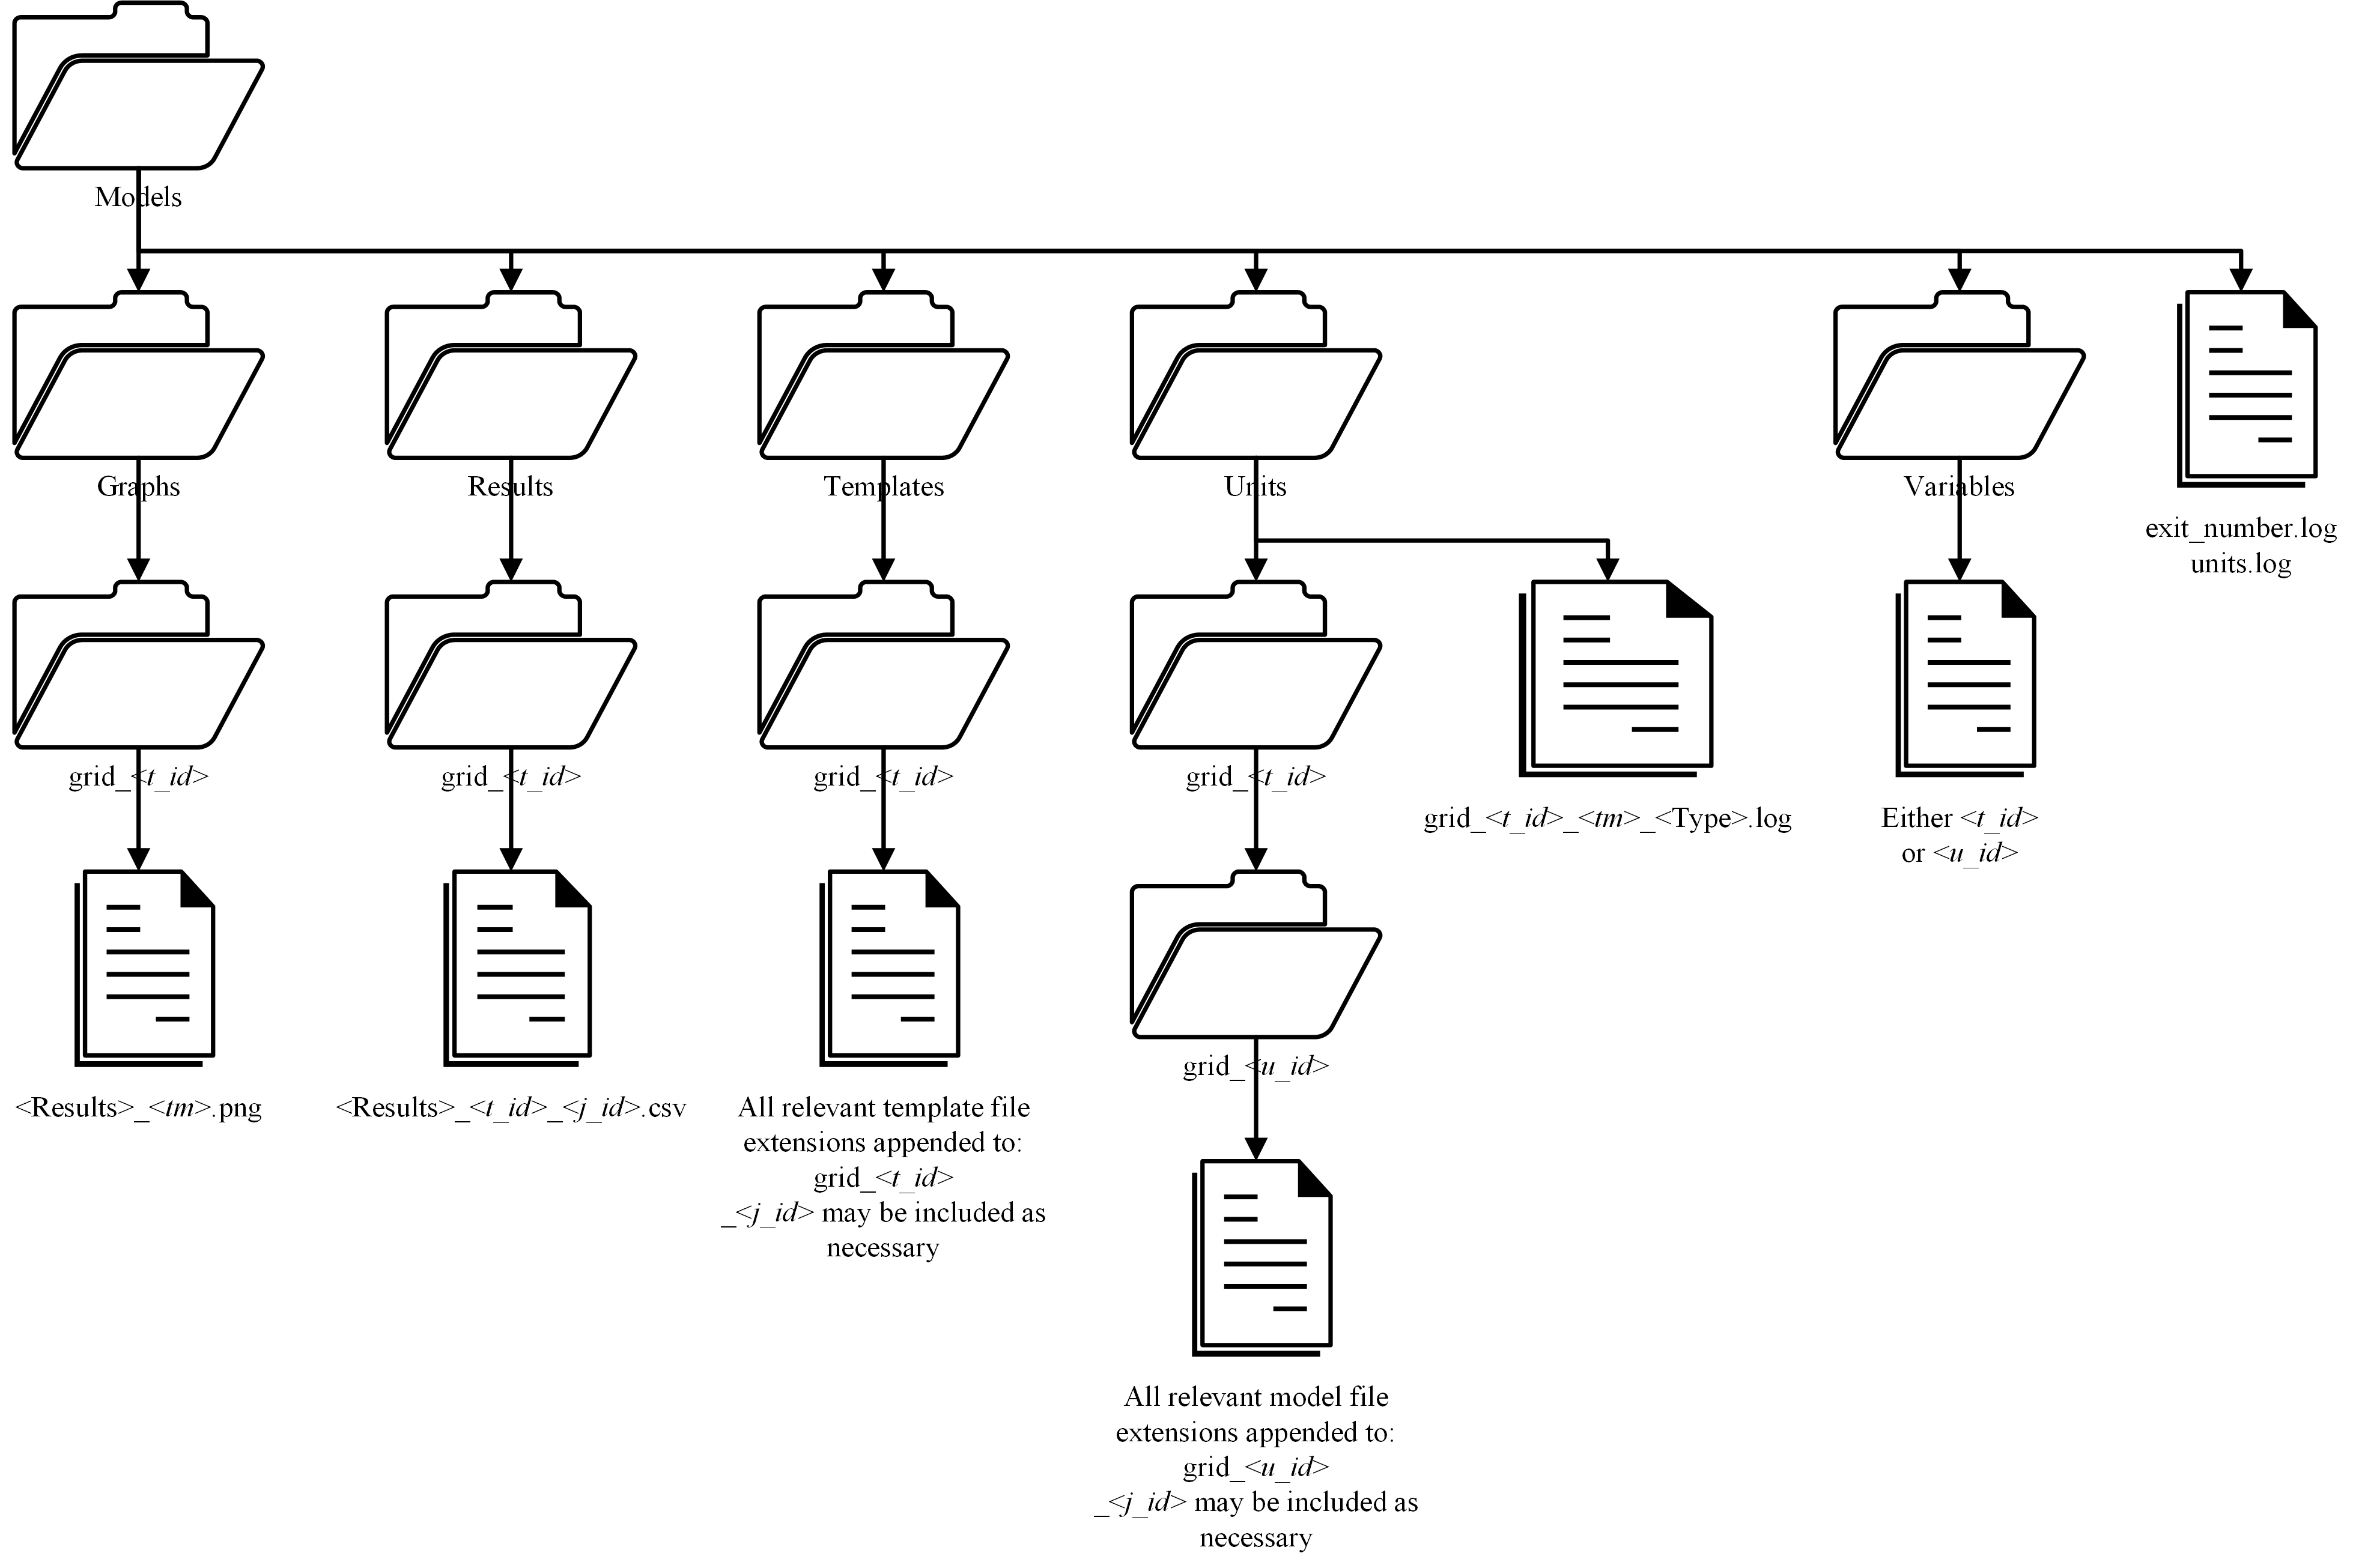
\includegraphics[width=1.4\textwidth]{FileHierarchy.png}
  \caption{File hierarchy flow diagram}
  \label{fig:fh}
 \end{figure}
\end{landscape}

% Please add the following required packages to your document preamble:
% \usepackage{booktabs}
\begin{table}[H]
\centering
\caption[File hierarchy parameters]{File hierarchy parameters and descriptions}
\label{tab:fhpar}
\begin{tabular}{@{}ll@{}}
\toprule
\multicolumn{1}{c}{\textbf{Parameter}} & \multicolumn{1}{c}{\textbf{Description}}              \\ \midrule
\textit{tm}                            & The timestamp of the simulation formatted as a string \\
\textit{t\_id}                         & The template ID                                       \\
\textit{u\_id}                         & The unit ID                                           \\
\textit{j\_id}                         & The job ID                                            \\
Results                                & The type of simulation results stored                 \\
Type                                   & The type of units logged                              \\ \bottomrule
\end{tabular}
\end{table}

The template ID is described in Section~\ref{ssec:tempcr}. The job ID refers to one of two jobs. The first job applies the unit deformation boundary conditions as described in Section~\ref{sec:UC}. The second job applies the internal pressure boundary conditions as described in Section~\ref{ssec:us}.

The unit ID is determined by the unit generation method. All unit IDs start with the number of elements removed followed by an underscore. If the unit generation method is random, a unique hash code is generated according to the list of element IDs that have been removed. If the unit generation method is an L-System, a unique hash code is generated according to the L-System rules. If the unit generation method is a CPPN, the unit ID is formatted as

\vspace{\baselineskip}

\centerline{<\textit{mod\_id}>\_<\textit{seed}>\_<\textit{scale}>\_<\textit{hl\_n}>\_<\textit{hl\_s}>\_<\textit{thresh}>}

\vspace{\baselineskip}

The type of units logged in the log files are one of six possible types:

\begin{itemize}
	\item No Type - All units
	\item success - All units that have run successfully
	\item failed - All units that have run unsuccessfully
	\item empty - All units that have no internal elements
	\item full - All units that have all internal elements
	\item ranked - All units ranked according to their fitness values
\end{itemize}